\documentclass[xcolor=table,8pt,a4paper]{beamer} 
\usepackage{subcaption}

\usepackage{xcolor}
%\definecolor{ultralightgray}{gray}{0.8}
\usepackage{hao}
%\usefonttheme{serif}
%\usepackage[T1]{fontenc}
%\usepackage{lmodern}
%\usepackage{mathpazo}
%\usepackage{kpfonts}
%\usepackage{mathptmx}
\usepackage{appendixnumberbeamer}


\definecolor{MedianBrown}{RGB}{119,95,85}
\definecolor{MedianLightBrown}{RGB}{235,221,195}
\definecolor{MedianLightBlue}{RGB}{148,182,210}
\definecolor{MedianOrange}{RGB}{221,128,71}
\definecolor{MedianLightOrange}{RGB}{216,178,92}
\definecolor{MedianUltraLightOrange}{RGB}{245,236,215}

\newenvironment<>{varblockdef}[2][0.9\textwidth]{%
    \begin{minipage}{#1}
    \begin{actionenv}#3%
        \def\insertblocktitle{#2}%
        \par%
        \usebeamertemplate{block begin}}
    {\par%
        \usebeamertemplate{block end}%
    \end{actionenv}
    \end{minipage}}

\newenvironment<>{varblock}[2][0.9\textwidth]{%
    \begin{minipage}{#1}
    \begin{actionenv}#3%
        \def\insertblocktitle{#2}%
        \par%
        \usebeamertemplate{block example begin}}
    {\par%
        \usebeamertemplate{block example end}%
    \end{actionenv}
    \end{minipage}}
%\setbeamercolor*{block title}{fg=white, bg=MedianOrange}
%\setbeamercolor*{block title example}{fg=white, bg=MedianLightOrange}
%\setbeamercolor*{block body}{bg=MedianUltraLightOrange}
%\setbeamercolor*{block body example}{bg=MedianUltraLightOrange}

\usetheme{metropolis}
%\setsansfont{Fira Sans}  % be sure to compile with XeLaTeX
%\setbeamerfont{theorem body}{family=\sffamily, series=Light} % 'Light' for thinner text

\definecolor{BlueTOL}{HTML}{222255}
\definecolor{BrownTOL}{HTML}{666633}
\definecolor{GreenTOL}{HTML}{225522}
\setbeamercolor{normal text}{fg=BlueTOL,bg=white}
\setbeamercolor{alerted text}{fg=BrownTOL}
\setbeamercolor{example text}{fg=GreenTOL}

% ---- Block colors (Metropolis-friendly) ----
\setbeamercolor{block title}{fg=white,bg=BlueTOL}
\setbeamercolor{block body}{fg=BlueTOL,bg=BlueTOL!6}

\setbeamercolor{block title alerted}{fg=white,bg=BrownTOL}
\setbeamercolor{block body alerted}{fg=BlueTOL,bg=BrownTOL!8}

\setbeamercolor{block title example}{fg=white,bg=GreenTOL}
\setbeamercolor{block body example}{fg=BlueTOL,bg=GreenTOL!8}

%%TABLE
\usepackage{multirow}
\newcommand*{\arraycolor}[1]{\protect\leavevmode\color{#1}}
\newcolumntype{A}{>{\columncolor{MedianLightOrange!30}}c}
\newcolumntype{B}{>{\columncolor{MedianLightBlue!30}}c}


\setbeamertemplate{footline}[frame number]{}

\usepackage{amsfonts, graphicx, ifthen, mathtools, bm, bbm}
\usepackage{amsmath, amssymb, amsthm}
\usepackage{ulem}
\usepackage{tikz}
\usepackage{fontawesome5}
\usepackage{natbib}
%\bibpunct{(}{)}{;}{a}{}{,}
%\usepackage{twemojis}

\newtheorem{proposition}{Proposition}
\newtheorem{assumption}{Assumption}

\theoremstyle{remark}
\newtheorem*{remark}{Remark}

\hypersetup{colorlinks,citecolor=cyan, urlcolor=cyan, linkcolor=black}

%Hello everyone, today I am going to talk about one of my paper. We will discuss estimation methods with multiple weighted networks, their upper bounds and minimax lower bounds. 
\title{From Single to Multiple Weighted Networks\\ {\small Estimation \& Minimax Rates}}
\date{\textit{Department of Statistics, University of Wisconsin-Madison}\\ 2026-02-13}
\author{\large Hao Yan $|$ Preliminary Exam\\}


\begin{document}

\maketitle

%Networks are ubiquitous across many domains. In neuroscience, functional brain networks are constructed from resting-state fMRI data by treating brain regions as nodes and correlations in their activity as edges. This enables quantitative understading of differences in connectivity patterns between healthy controls and patient populations.
\begin{frame}{Motivation: Multiple Networks Modeling}
    \begin{itemize}
        \item \textbf{Networks are ubiquitous}
        across neuroscience, economics, social science, and genomics.
        \pause
        \begin{figure}
            \centering
            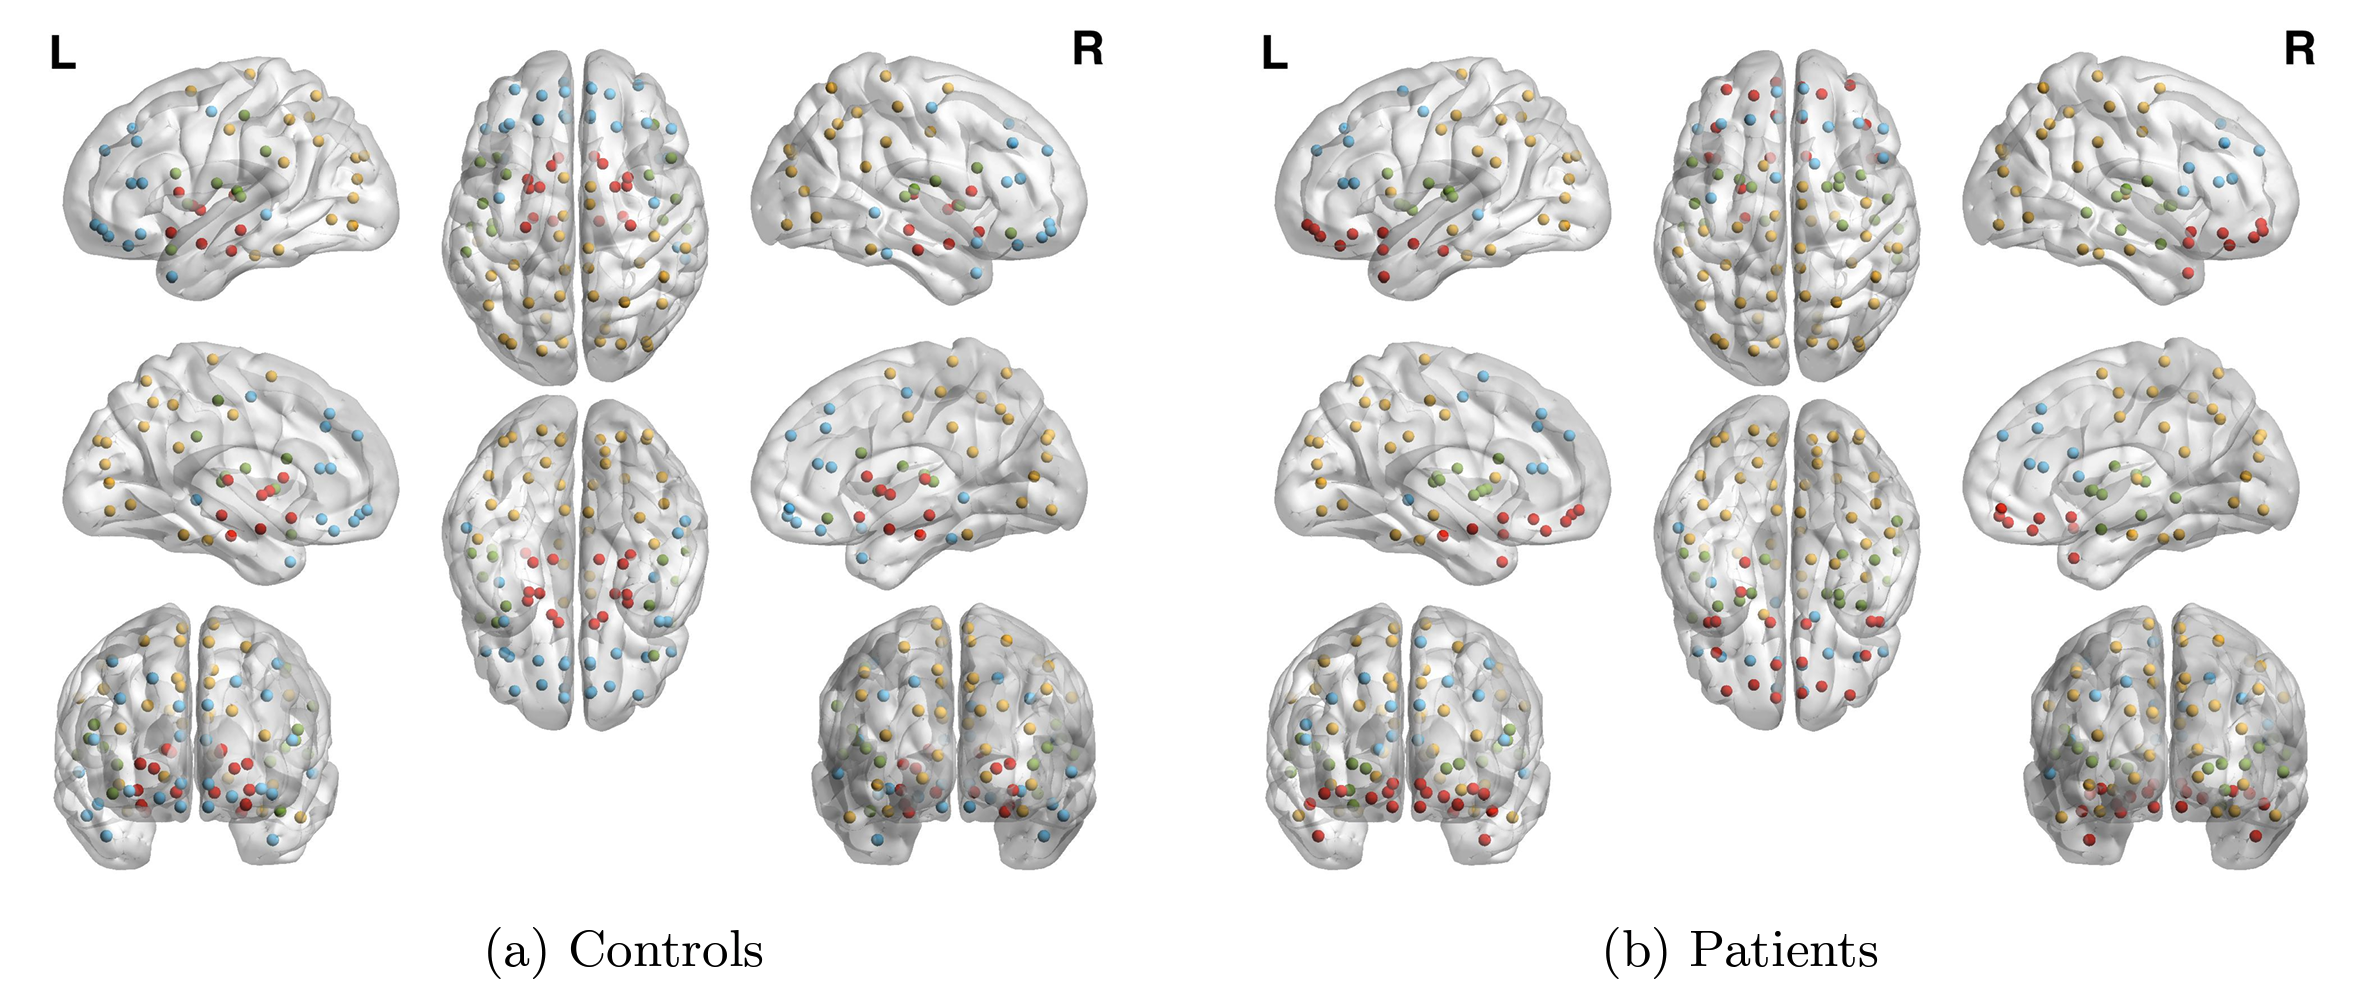
\includegraphics[width=\linewidth]{figs/brains.png}
            \caption{\textbf{Functional brain networks from resting-state fMRI.}
Brain regions (atlas-defined) are nodes, and edges are defined by thresholded correlations between resting-state fMRI time series.
Data are from the publicly available COBRE schizophrenia dataset \citep{paul2020random}.}
        \end{figure}
    \end{itemize}
\end{frame}


%In economics, networks provide a natural way to study international trade: here, countries are nodes and edges encode trade intensity, with separate networks over the same set of countries representing different categories of traded agricultural products.
\begin{frame}{Motivation: From Single to Multiple Networks}
    \begin{itemize}
        \item \textbf{Networks are ubiquitous}
        across neuroscience, economics, social science, and genomics.
        \begin{figure}
            \centering
            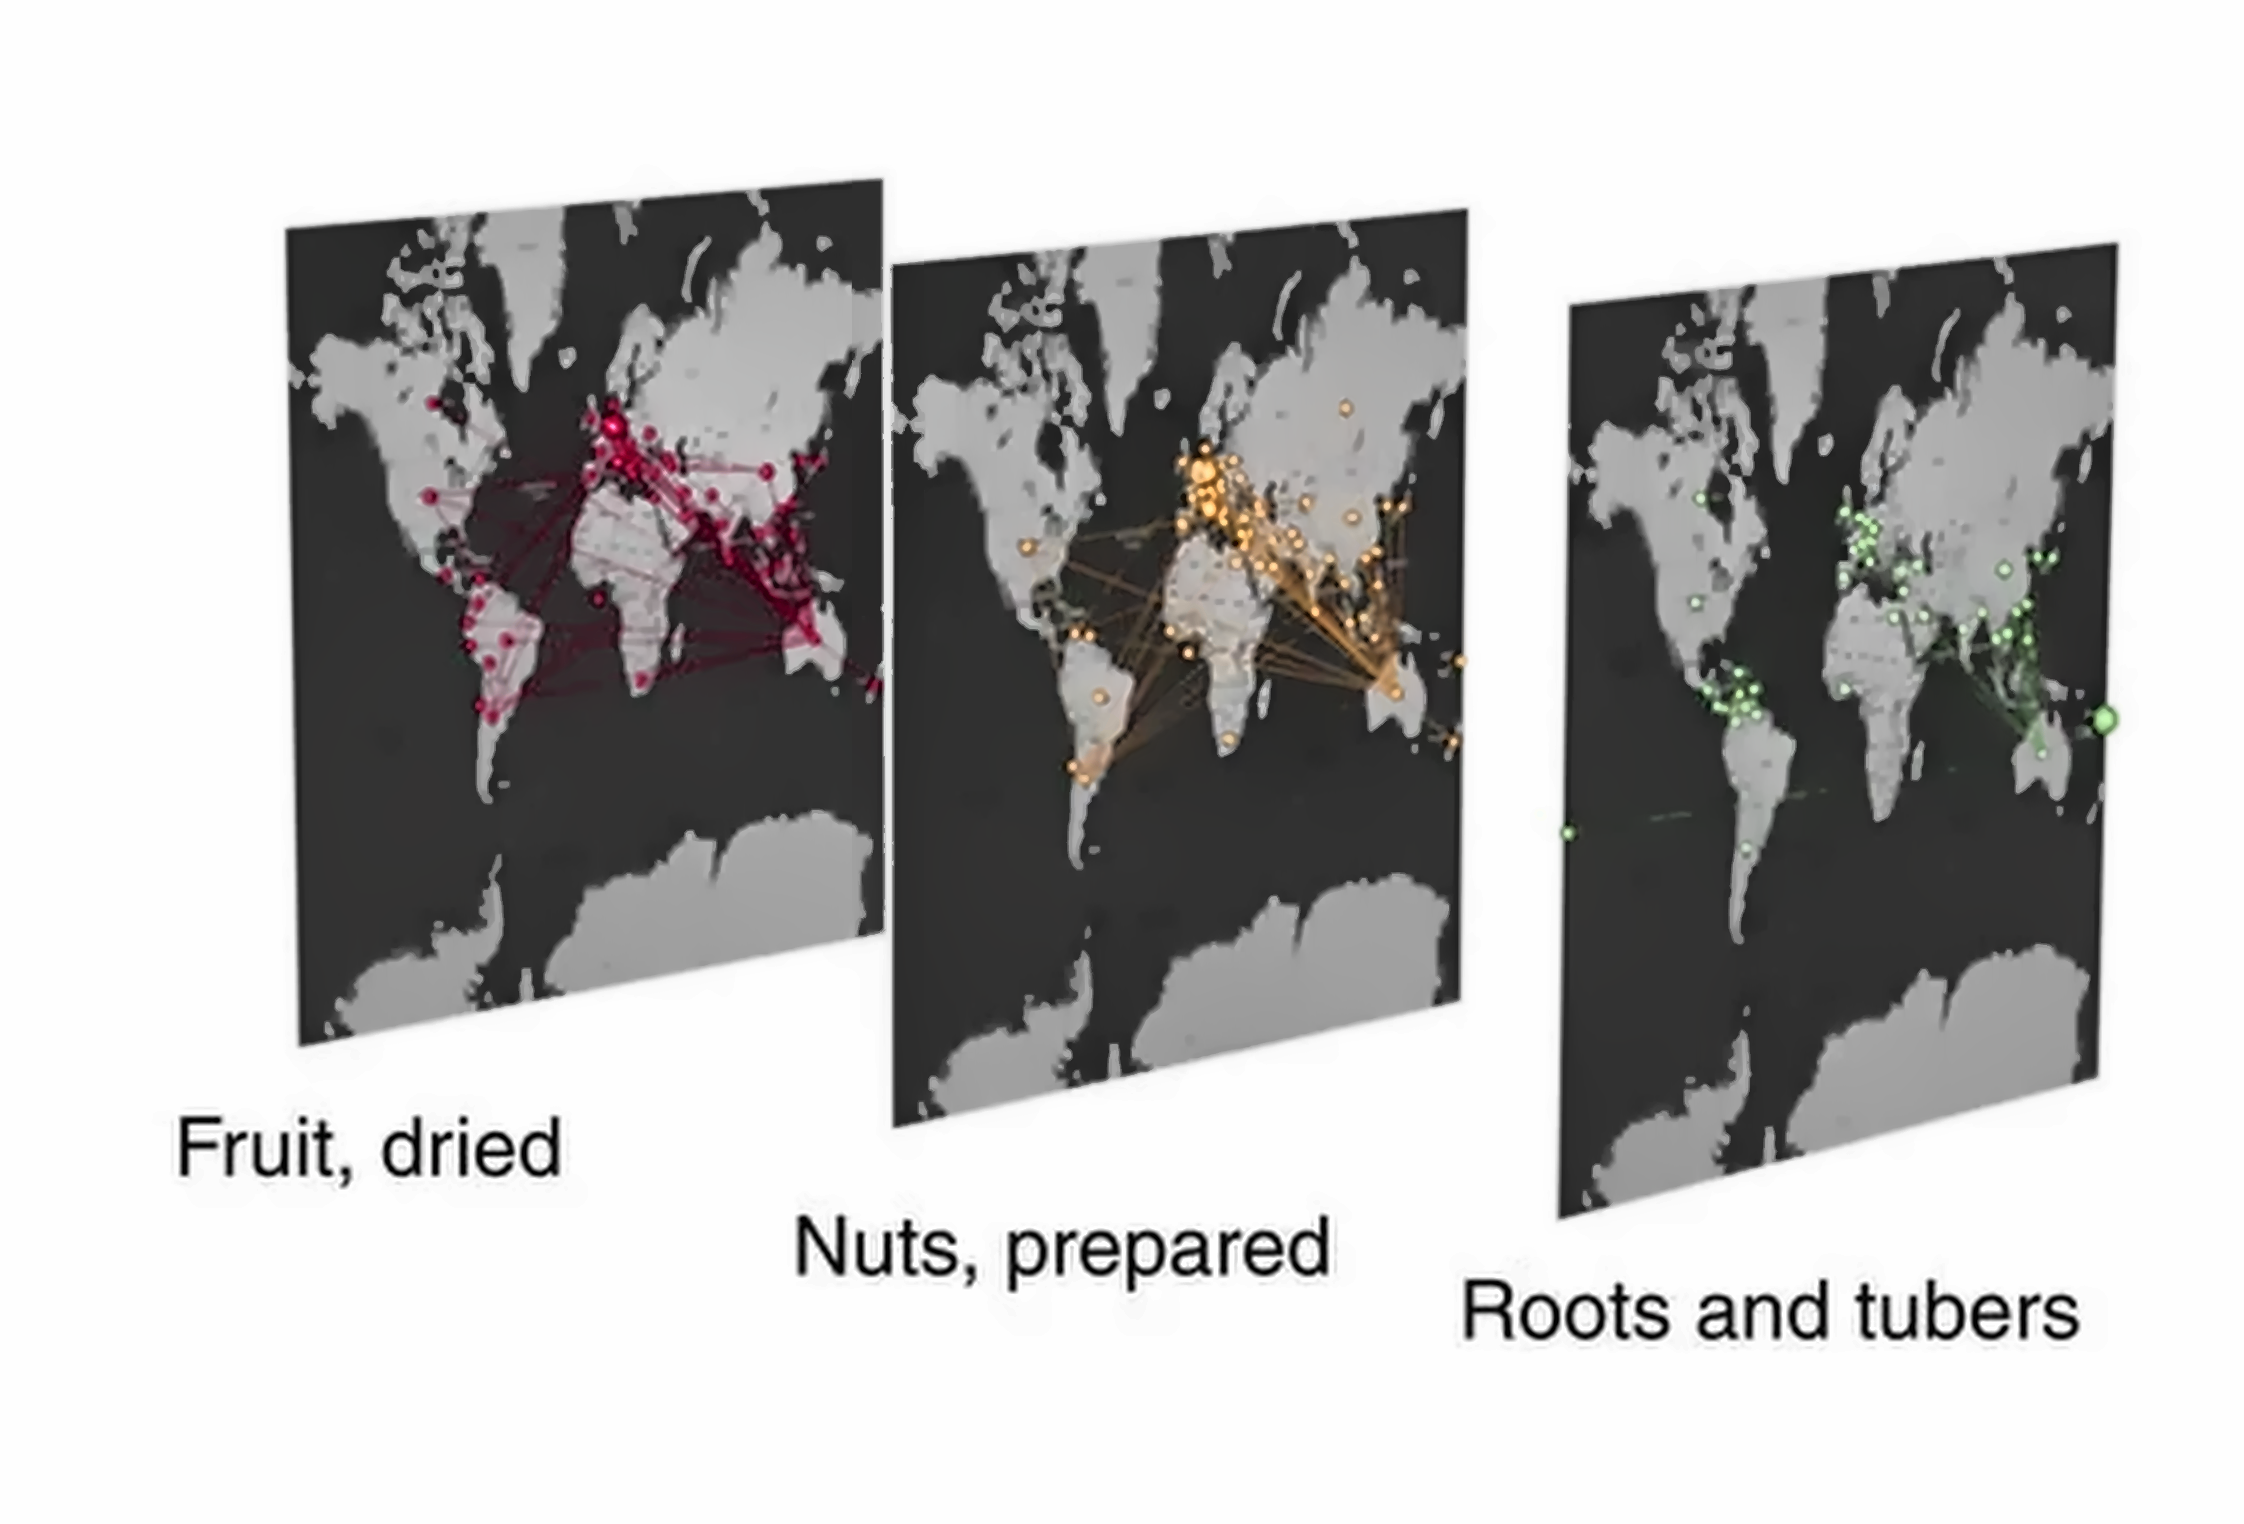
\includegraphics[width=0.8\linewidth]{figs/figure_b_slide_cleaner_maps_v4_no_ocean_labels.png}
            \caption{\textbf{ FAO worldwide food import/export network.} Food and agriculture trade relationships between countries \citep{de2015structural}. Each node corresponds to a country, and each layer to a different agricultural product. The undirected edges are
weighted by the bilateral traded quantity of the commodity. }
        \end{figure} %TODO: crop out the distance matrix thing, because it is irrelevant to what we want to focus on here.
    \end{itemize}
\end{frame}



% There is a rich literature on statistical network models, traditionally focused on a single observed network, including classical frameworks such as stochastic block models, latent space models, and some other related approaches.
% In modern datasets, as illustrated by the previous examples, we often observe multiple networks defined on a common set of nodes, which can be viewed as noisy realizations of an underlying latent structure.
% There are also many direct extensions of classical single-network models to the multiple-network setting, where a common theme is that the networks share a low-rank common structure while also exhibiting low-rank, network-specific variation.
% This naturally raises two questions: first, most low-rank modeling approaches induce global differences across networks—what if the differences instead have a sparse structure? We address this in our paper but I will only briefly talk about it at the end of this talk. The second question is that, if the networks are simply independent replications, can having multiple networks still provide any nontrivial statistical benefit? So I will be focusing on the second question in this talk. I will talk about estimation methods and optimality under multiple observations. 
\begin{frame}{Motivation: From Single to Multiple Networks}

    \begin{itemize}
        %\item \textbf{Networks are ubiquitous}
        %across neuroscience, economics, social science, and genomics.
        %\begin{itemize}
            %\item Nodes are often \textbf{aligned across subjects, conditions, or time}.
        %\end{itemize}
        \item \textbf{Modern data: multiple networks}
        \begin{itemize}
            \item Repeated observations on a common node set.
            \item Viewed as \textbf{multiple noisy copies of some underlying structures}.
        \end{itemize}
        
        \item \pause \textbf{Classical models:}
        SBMs \citep{holland1983stochastic, airoldi2008mixed}, Latent space models \citep{hoff2002latent}, RDPGs \citep{YouSch2007}, Graphons \citep{Lovasz2012}
            %\item Inference from \textbf{one noisy matrix}.

        \item \pause \textbf{Prior work: shared low-rank or community structure}
        \begin{itemize}
            \item Multilayer SBMs \citep{lei2023bias, lei2024computational}
            \item Multiplex Latent Space Model \citep{macdonald2022multiness}
            \item Multiple RDPG \citep{nielsen2018multiple, arroyo2021inference, levin2022recovering}
        \end{itemize}

        %TODO: I think it would be clearer to split this into two slides: one about prior work, and one talking about open questions and what we are going to talk about here.

        \item \pause \textbf{Questions} %TODO: clarify that we do both of these things in the paper; we are going tofocus on the replication one here today; but we'll talk briefly about sparse differences at the end
        \begin{itemize}
            \item Variations between different observations \\
            \pause Existing work leads to dense differences—what about \textbf{sparse difference structures}?
            \item \pause When does replication help, and which \textbf{structural features} benefit the most?
        \end{itemize}

        \item \pause \textbf{In this talk}
        \begin{itemize}
            \item Start from a shared low-rank model. 
            \item Study how \textbf{multiple observations} improve estimation, what estimation method, optimality. 
        \end{itemize}

        %\item \pause \textbf{Key question:}
        %How does having \textbf{multiple observations} improve estimation
        %    of the underlying network structure?
    \end{itemize}

\end{frame}


%\begin{frame}{Existing Work and the Modeling Gap}

%    \begin{itemize}
%        \item \textbf{Prior work on multiple networks}
%        \begin{itemize}
%            \item Joint embeddings and multilayer SBMs.
%            \item Assumes a \textbf{shared low-rank or community structure}.
%        \end{itemize}

 %       \item \pause \textbf{Main emphasis}
 %       \begin{itemize}
 %           \item Pooling information to estimate a \textbf{common latent structure}.
 %           \item Differences treated as smooth or low-rank variations.
 %       \end{itemize}

  %      \item \pause \textbf{Open issue}
  %      \begin{itemize}
  %          \item Less is understood about \textbf{when replication helps}
  %          and \textbf{what aspects of structure benefit most}.
  %      \end{itemize}

   %     \item \pause \textbf{Our approach}
   %     \begin{itemize}
   %         \item Start from a shared low-rank model.
   %         \item Study how \textbf{multiple observations} improve estimation,
   %         and when additional structure becomes identifiable.
   %     \end{itemize}
   % \end{itemize}

%\end{frame}

% We assume access to K symmetric weighted networks defined on a common set of n nodes. We denote their adjacency matrix as Ys. 
% And we assume Ys follows a signal plus noise model Mstar + Ws, Ws are independent mean zero noise matrices, and Mstar is a shared signal matrix. Its rank r is assumed to be much smaller than the matrix dimension n, and throughout the talk, we will treat it as a constant, and assume it is known to us. We write the spectral decomposition of Mstar as Ustar Lambdastar Ustar transpose. We will be primarily focusing on estimating Ustar from multiple observations.  
\begin{frame}{Problem Setup: Multiple Observations of a Low-Rank Matrix}

    \begin{itemize}
        \item \textbf{Data:}
        observe \( K \) symmetric weighted networks
        \[
        \{\mY_s \in \mathbb{R}^{n \times n} : s = 1,\dots,K\},
        \]
        defined on a common set of \( n \) nodes.

        \item \pause \textbf{Model:}
        each network is a noisy observation of a shared signal
        \[
        \mY_s = \mM^\star + \mW_s, \qquad s = 1,\dots,K
        \]
        \item \pause \textbf{Signal assumption:}
        the shared signal is low rank,
        \[
        \mathrm{rank}(\mM^\star) = r \ll n, %TODO: be prepared to answer questions about whether r is known
        \quad
        \mM^\star = \mU^\star \mLambda^\star (\mU^\star)^\top
        \]
        \item \pause \textbf{Noise assumption:} \( \mW_s \) are independent, mean-zero noise matrices
        \begin{itemize}
            \item \pause \textbf{(Heteroscedastic variance)} \; 
            $
                \mathbb{E}[W_{s, ij}^2]
                \;=\;
                \sigma_{ij}^2
                \;\le\;
                \sigma^2.
            $
        \item \pause \textbf{(Boundedness)} \;
        $
            |W_{s, ij}| \;\le\; L,
            \; \text{with high probability.}
        $
        \end{itemize}
    \end{itemize}
    \pause
    \begin{alertblock}{Goal}
        Estimate $\mLambdastar$ and $\mUstar$ from multiple noisy observations,
and understand how \textbf{independent replications} improve estimation beyond a single copy.
    \end{alertblock}

\end{frame}

% One baseline we can compare to is averaging. Let Ybar be the average of all observations, this would reduce the noise variance by a factor of K. We can then treat Ybar as a single observation, and use the top eigenvectors and eigenvalues to perform estimation. This approach is already minimax optimal, under metrics such as frobenius norm and operator norm.  
% The takeaway message is that under norms that consider all entries, multiple observations only plays variance reduction role.
\begin{frame}{Classical Global Losses: Frobenius \& Operator Norms}

\begin{itemize}

    \item \textbf{Averaging baseline:}
    \[
        \bar{\mY} := \frac{1}{K}\sum_{s=1}^K \mY_s
        = \mM^\star + \bar{\mW},
        \qquad \operatorname{Var}\left(\bar{W}_{ij}\right) \leq \sigma^2/K.
    \]
    \item \pause \textbf{Spectral Decomposition} 
    $$
        \bar{\mY} = \mU_{\mathrm{sp}}  \mLambda \mU_{\mathrm{sp}}^\top + \mU_{\perp} \mLambda_{\perp} \mU_{\perp}^\top
    $$
    \item \pause \textbf{Frobenius norm (Schatten-2):} minimax optimal \hfill \citep{koltchinskii2011nuclear}
    \[
        \inf_{\hat{\mM}}
        \sup_{\mathrm{rank}(\mM^\star)\le r}
        \mathbb{E}\|\hat{\mM}-\mM^\star\|_F^2
        %\asymp \bar{\sigma}^2 r n 
        \asymp \frac{\sigma^2}{K} rn.
    \]
    

    %\item \pause \textbf{Operator norm (Schatten-\(\infty\)):} minimax optimal \hfill \citep{tropp2012user,vershynin2018high}
    %\[
    %    \inf_{\hat{\mM}}
    %    \sup_{\mathrm{rank}(\mM^\star)\le r}
    %    \mathbb{E}\|\hat{\mM}-\mM^\star\|
    %    \asymp \bar{\sigma}\sqrt{n}.
    %\]
    
    \item \textbf{Subspace Estimation: } minimax optimal \hfill \citep{cheng2021tackling}
    \[
        \inf_{\hat\mU} \sup_{\mMstar: \lambdastar_r - \lambdastar_{r+1} \geq \Delta} \E \min_{\mO \in \mathbb{O}(r)}
        \bigl\|\widehat{\mU}\mO - \mU^\star\bigr\|
        %\;\lesssim\;
        %\frac{\bar{\sigma} \sqrt{n}}{\lambda_r^\star} 
        \asymp \min\left\{\frac{\sigma}{\sqrt{K}} \cdot \frac{\sqrt{n}}{\Delta}, 1\right\}.
    \]
    \small The orthogonal alignment accounts for rotational ambiguity.
    \pause
    \begin{alertblock}{Takeaway}
        Under \emph{global} norms, multiple observations play a trivial
    \emph{variance-reduction role}
        %\item averaging improves constants, but yields no additional structural gain.
    \end{alertblock}
\end{itemize}

\end{frame}


%\begin{frame}{Estimation Targets and Error Metrics}

%\begin{itemize}
    %\item \textbf{Low-rank matrix estimation (shared structure)}
    %\begin{itemize}
    %    \item \textbf{Row-wise error:} 
    %    $$
    %    \left\|\widehat{\mM}-\mM^\star\right\|_{2,\infty} := \max_{i\in[n]} \left\|(\widehat{\mM}-\mM^\star)_{i,\cdot}\right\|_2 
    %    $$
        % row-wise bound for \Delta
    %    \item \textbf{Entrywise error:}\ 
    %    $$
    %    \left\|\widehat{\mM}-\mM^\star\right\|_{\infty} := \max_{i,j} \left|\widehat{M}_{ij}-M^\star_{ij}\right|
    %    $$
    %\end{itemize}

    %\item \textbf{Linear functionals of eigenvectors}
    %\begin{itemize}
    %    \item For fixed \(\va\) with \(\|\va\|_2=1\):\ 
    %    $$
    %    \left| \va^\top \widehat{\vu}_\ell - \va^\top \vu^\star_\ell \right|
    %    $$
    %    \item \textbf{Entrywise eigenvector control:}\ 
    %    $$
    %    \left\|\widehat{\vu}_\ell \pm \vu^\star_\ell\right\|_\infty
    %    $$
    %\end{itemize}

    %\item \pause \textbf{Eigenspace / subspace estimation}
    %    $$
    %    \min_{\mO\in\mathbb{O}(r)} \|\widehat{\mU}\mO-\mU^\star\|_{2,\infty}
    %    $$
    
%\end{itemize}

%\end{frame}



%Before we have further discussion, we need to make our assumptions on the noise matrix W more explicit. 
% We allow heteroscedastic variance, as long as they satisfy a uniform upper bound given by sigma2. We assume the noise magnitude is bounded by L. L is not a constant, it can depends on quantities such as matrix dimension n and variance sigma2. We impose a technical condition on the range of L. This mu is the incoherence parameter, which we will talk about in the next slide. 
% And we assume the noise is symmetric about 0. 


\begin{frame}{Warmup: Row-wise Bound for Spectral Estimator}
\small

% =====================================================
% Top: theory (fixed position across all overlays)
% =====================================================
\begin{overlayarea}{\textwidth}{0.34\textheight}
\vspace{-2em}
\begin{itemize}
  \item<1-> \textbf{Spectral estimator (single observation).}
  When $\lambdastar_{\min} \gtrsim \sigma \sqrt{n}$,
  \vspace{-0.3em}
  \[
    \left\|\boldsymbol{U}_\mathrm{sp}
    \operatorname{sgn}(\mU^\top_\mathrm{sp}\mUstar)
    - \boldsymbol{U}^{\star}\right\|_{2,\infty}
    = \tilde{O}\!\left(\frac{\sigma \sqrt{\mu}}{\lambdastar_{\min}}\right),
    \hfill \quad\text{\citep{chen2021spectral}}.
  \]
  \vspace{-1.2em}
  \item<2-> \textbf{Coherence (eigenspace localization).}

  % show on <2->, reserve identical height on <1>
  \onslide<2->{
  \vspace{-0.6em}
  \[
    \mu
    := \frac{n}{r}\,\|\mU^\star\|_{2,\infty}^2
    = \frac{n}{r}\max_{i\in[n]}\|\mU^\star_{i,\cdot}\|_2^2,
    \qquad 1 \le \mu \le \frac{n}{r}.
  \]
  }
  \onslide<1>{
  \[
    \vphantom{
    \mu
    := \frac{n}{r}\,\|\mU^\star\|_{2,\infty}^2
    = \frac{n}{r}\max_{i\in[n]}\|\mU^\star_{i,\cdot}\|_2^2,
    \qquad 1 \le \mu \le \frac{n}{r}.
    }
  \]
  }
\end{itemize}
\end{overlayarea}
% =====================================================
% Bottom: staged real-data -> empirical -> theory
% =====================================================

\begin{overlayarea}{\textwidth}{0.44\textheight}

% ---------- <3>: hubs statement + network plot ----------
\only<3>{
\vspace{-4.8em}
\begin{figure}
\hspace*{-1cm}
\begin{tikzpicture}
    \node[inner sep=0] (img) 
        {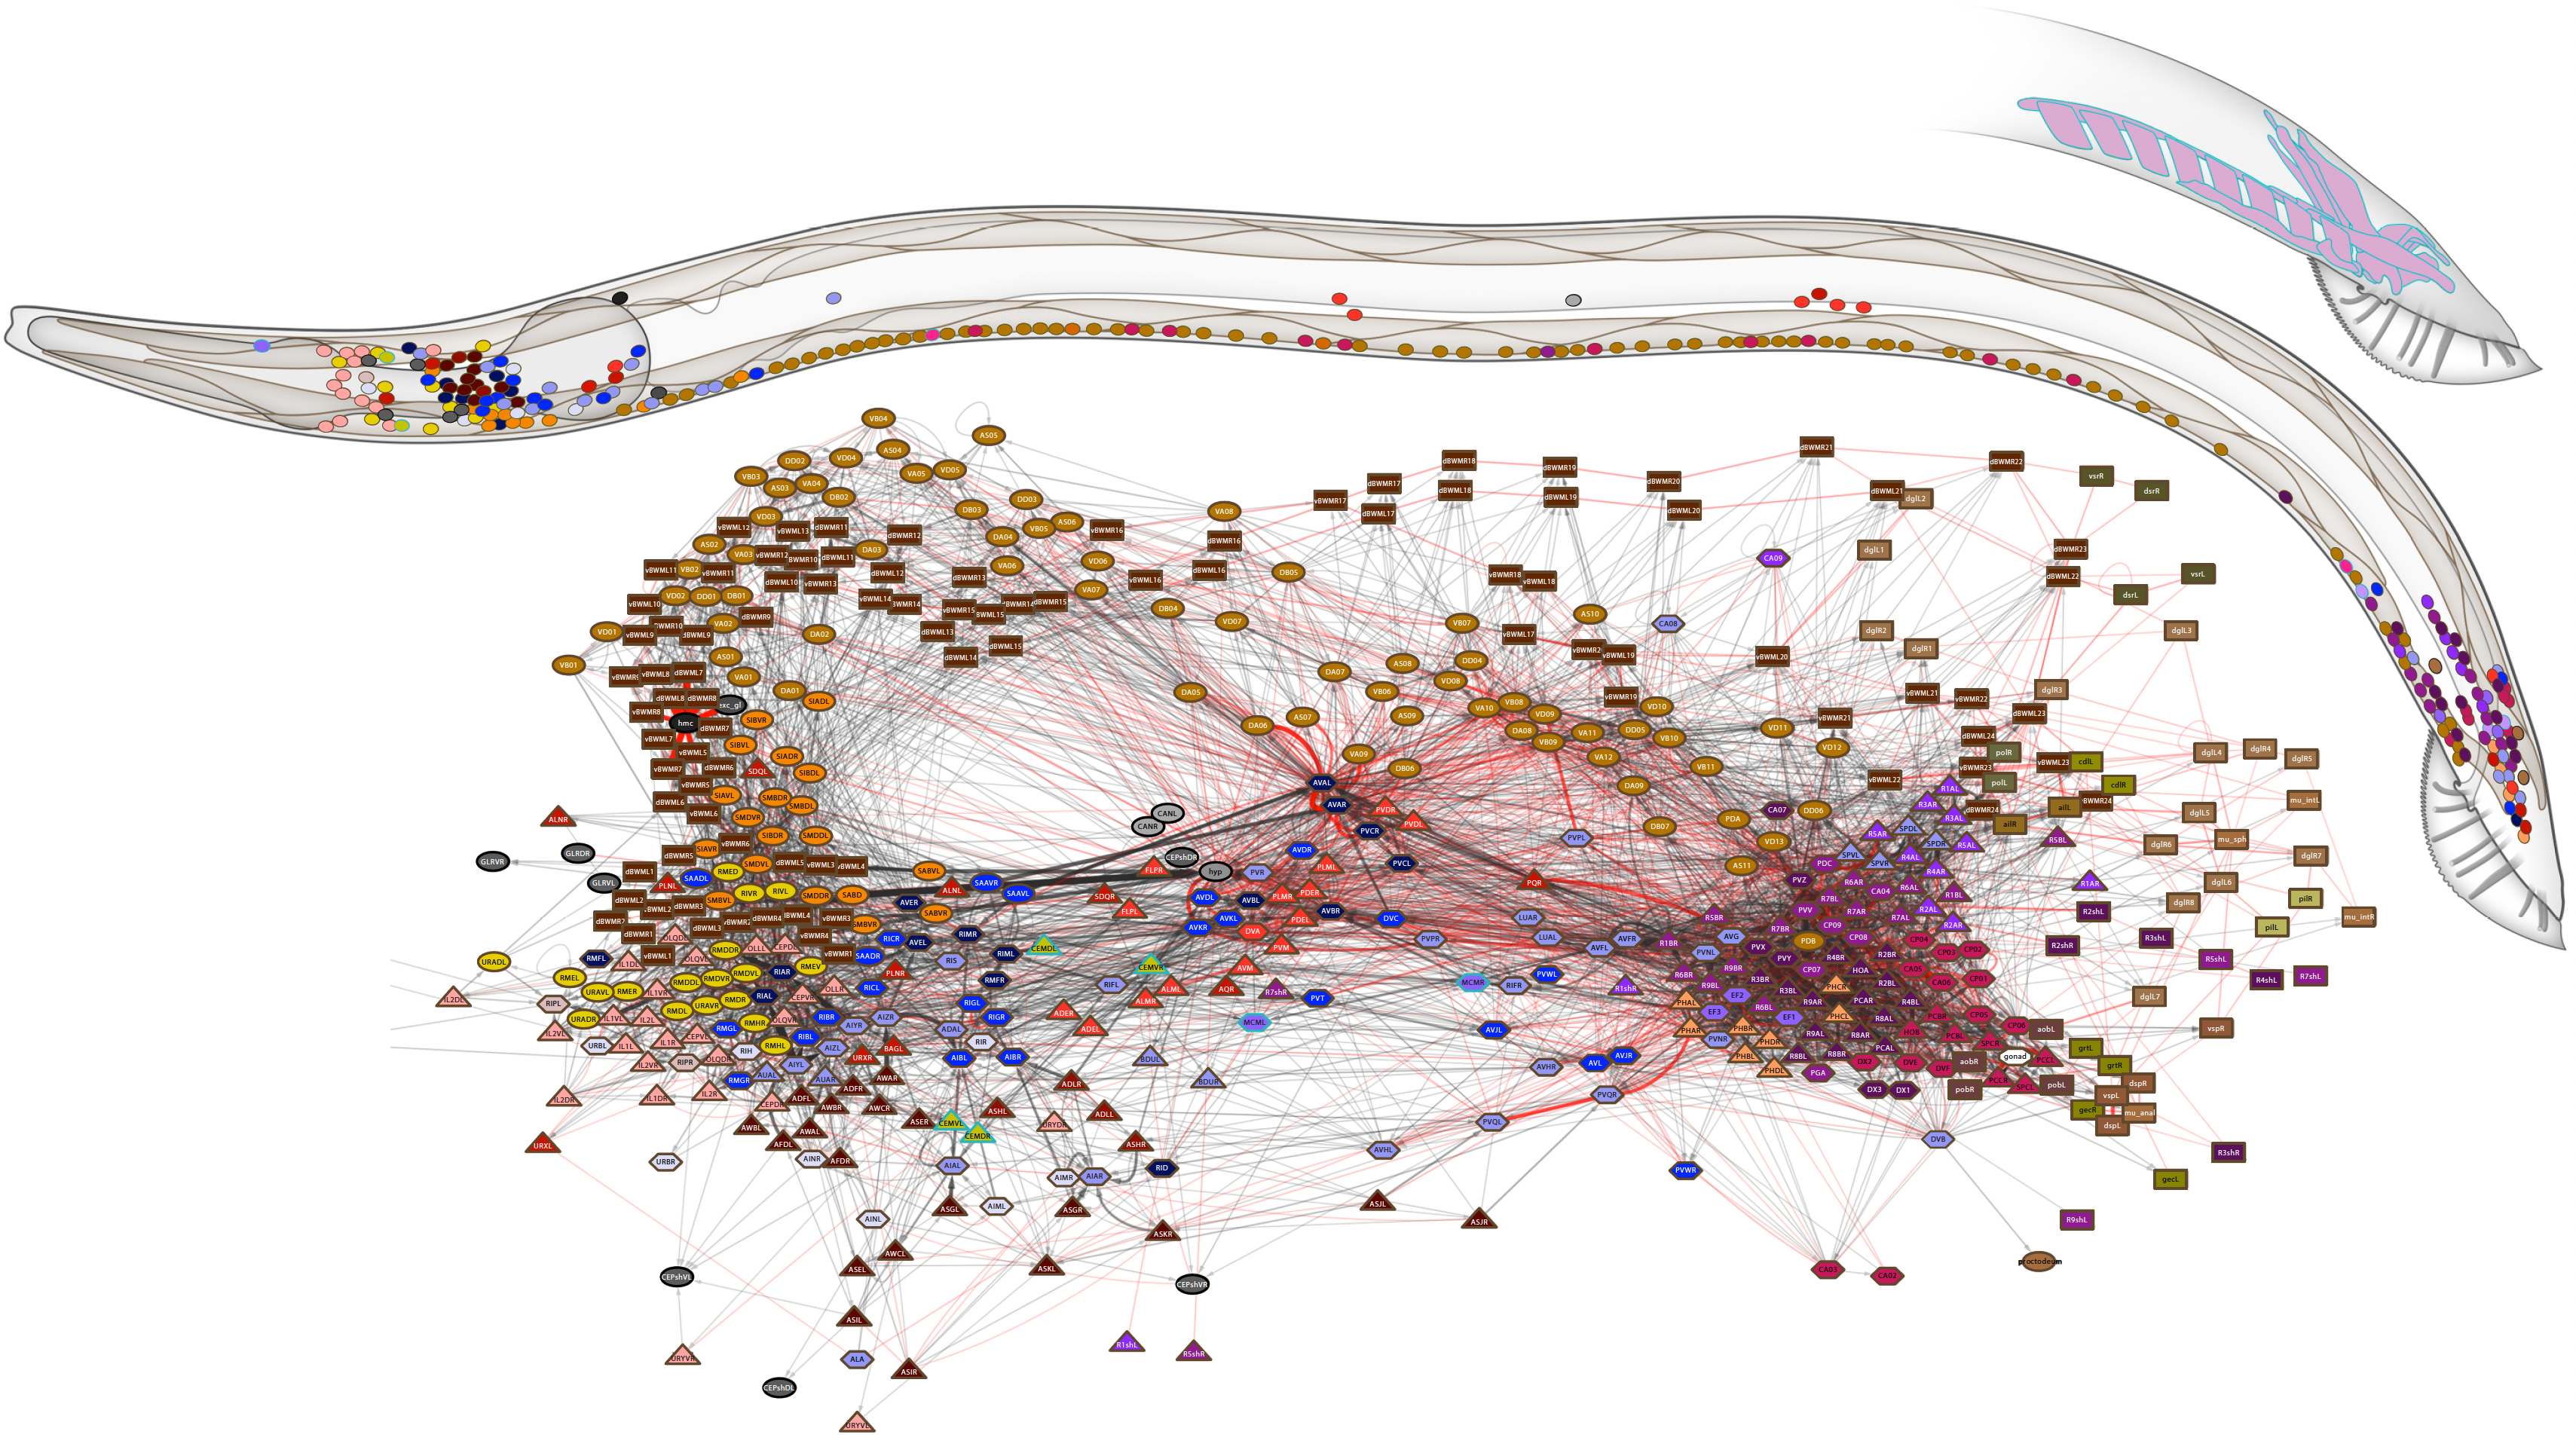
\includegraphics[width=0.9\linewidth]{figs/celegans_connectome.png}};
    
    % Adjust x/y to move text into white area
    \node[align=left, text width=0.45\linewidth] 
        at ([xshift=-2.7cm,yshift=2.5cm]img.center)
    {
        \fbox{\textcolor{teal}{\textbf{Real network has hubs}}}
    };

    \node[align=left, text width=0.2\linewidth] 
        at ([xshift=-4.cm,yshift=-0.45cm]img.center)
    {
        \footnotesize Adult \emph{C. elegans} chemical synapse connectome
    };
\end{tikzpicture}
\end{figure}
}

% ---------- <4>: keep hubs statement + add dataset details; keep network plot ----------
%\only<4>{
%\vspace{-4em}
%\begin{beamercolorbox}[rounded=true,shadow=true,sep=0.4em]{block body}
%\vspace{-1.5em}
%\begin{columns}[T,onlytextwidth]

%\begin{column}{0.44\textwidth}
%\begin{itemize}
%  \item \textbf{Dataset (connectome).}
%  \begin{itemize}
%    \item Adult \emph{C. elegans} hermaphrodite chemical synapse connectome
%    (directed, weighted adjacency $\mA$; \citep{cook2019wholeanimal}).
%    \item Neuron--neuron block: $n \approx 300$.
%    An edge $A_{i j}$ represents the number of chemical synapses from neuron $i$ to neuron $j$.
%  \end{itemize}
%\end{itemize}
%\end{column}

%\begin{column}{0.54\textwidth}
%\vspace{-0.2em}
%\begin{figure}
%  \centering
%  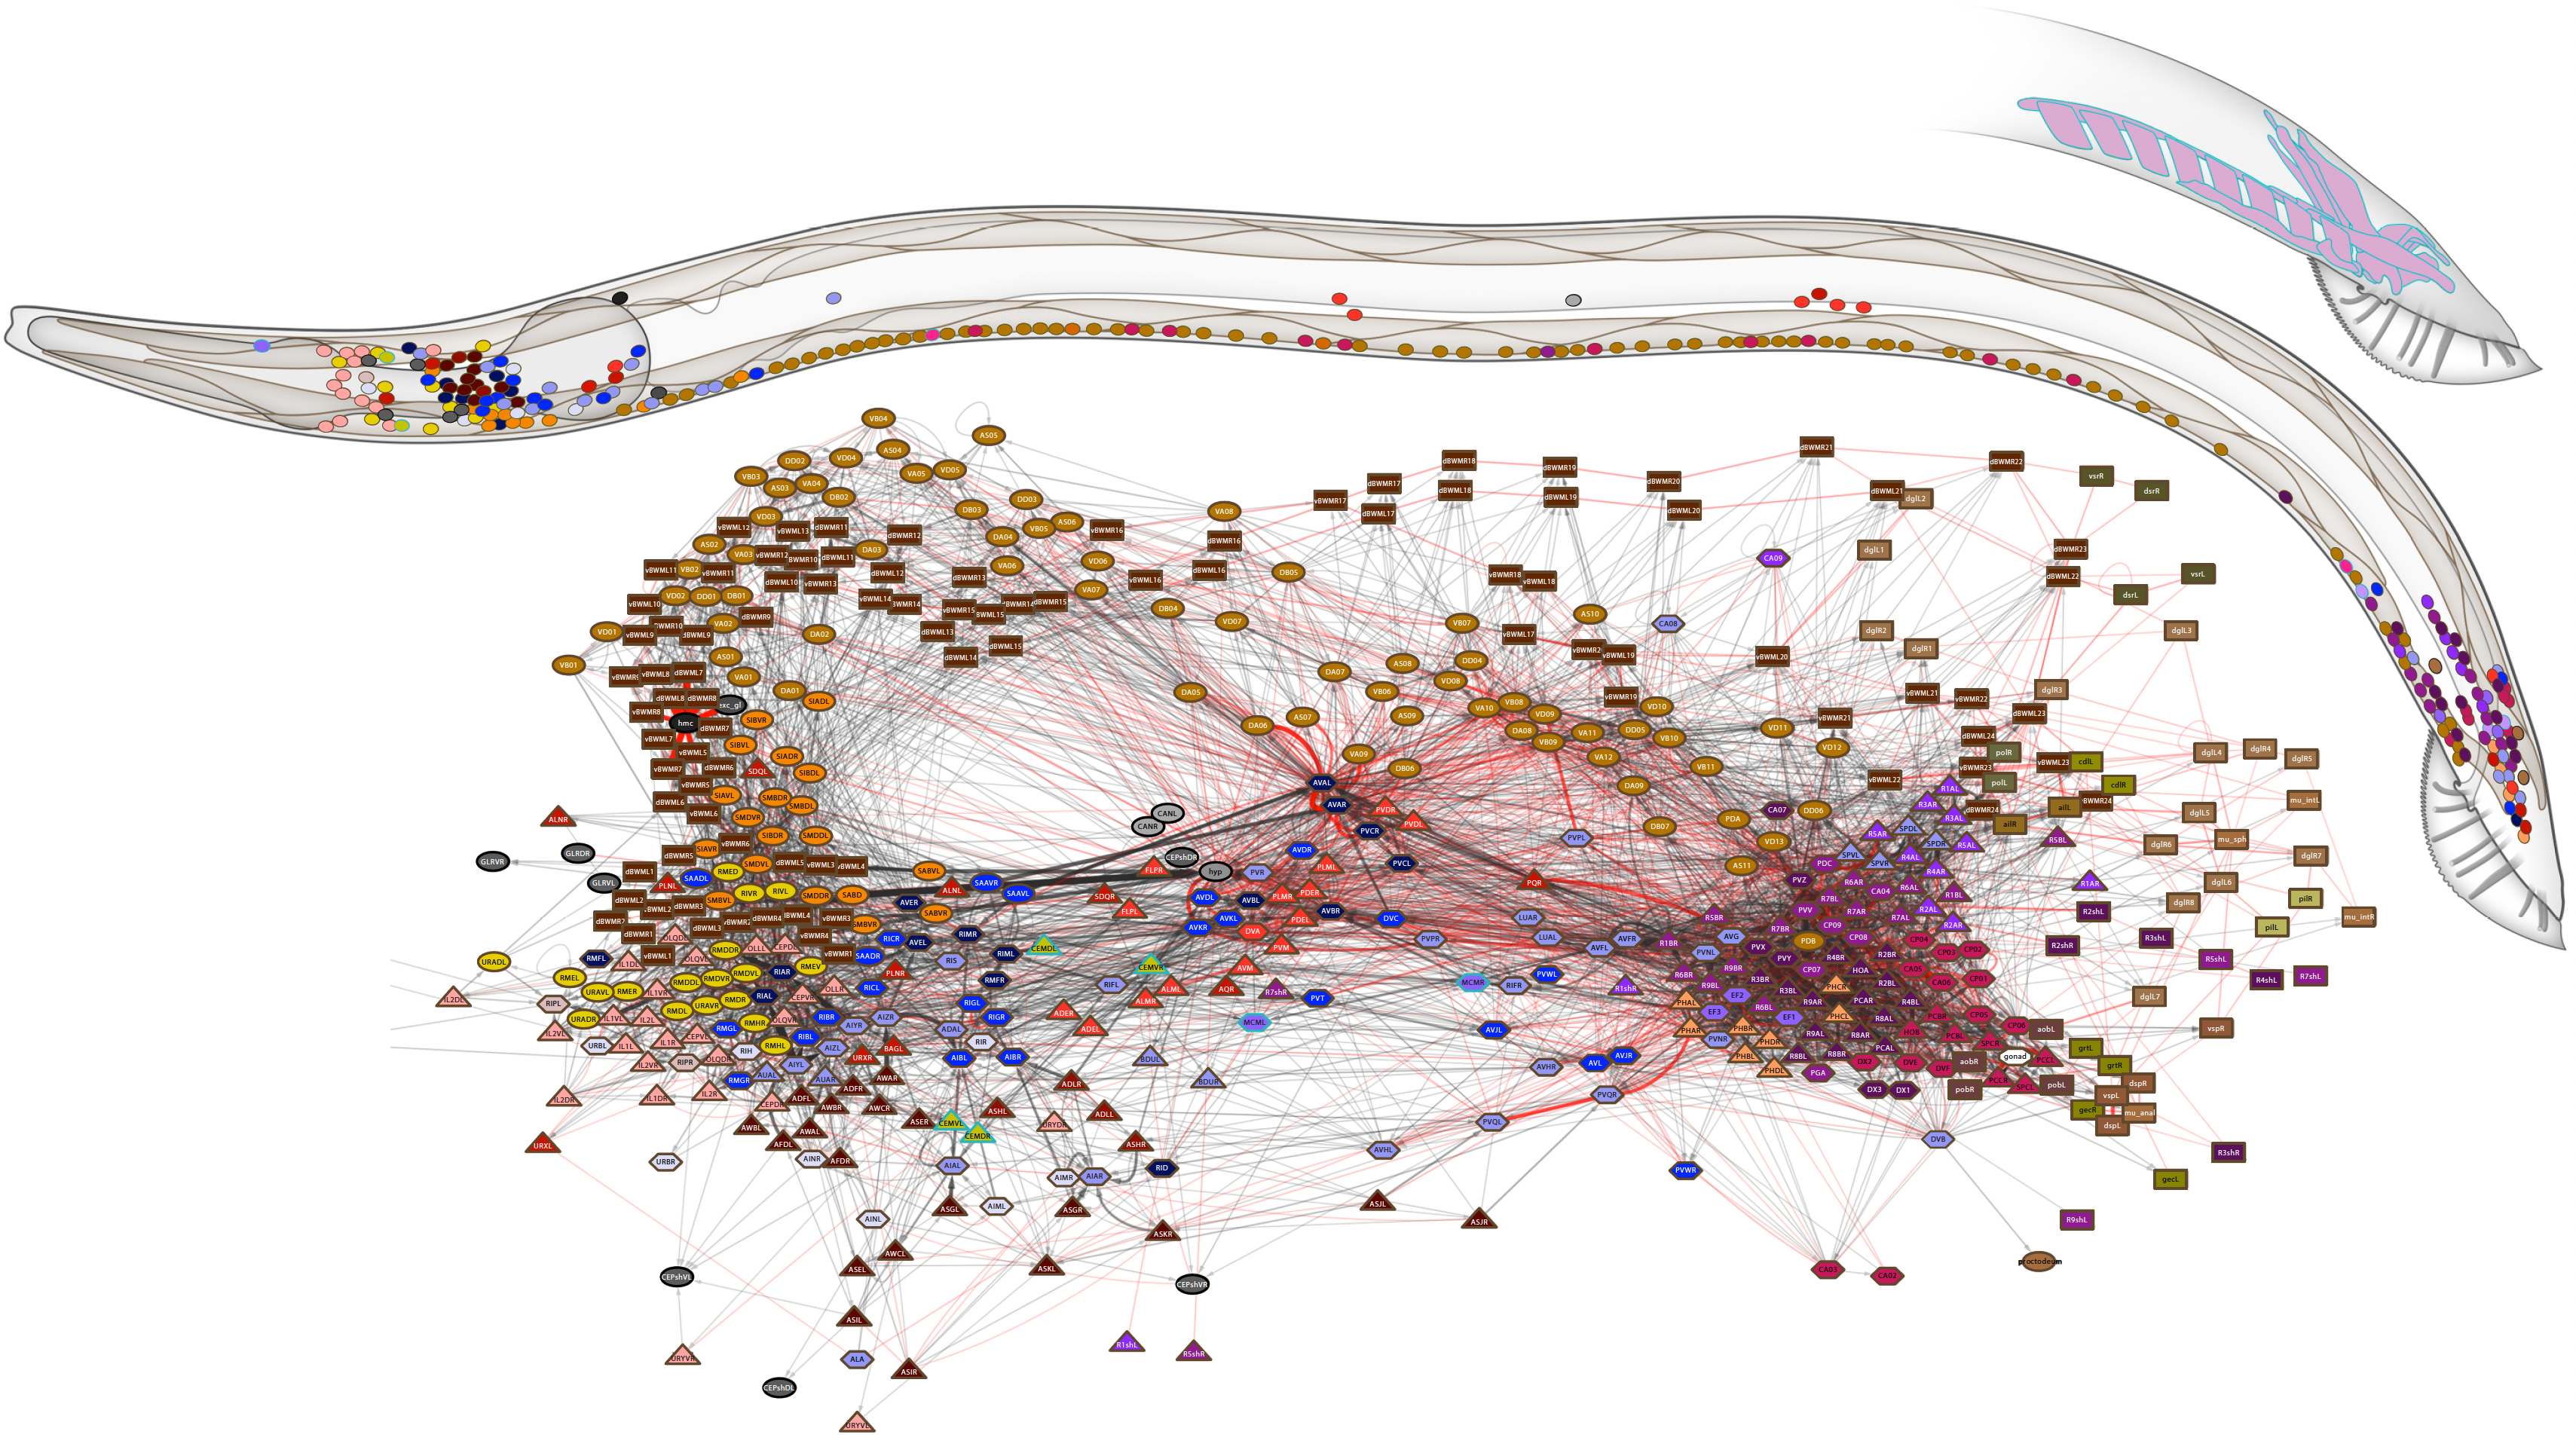
\includegraphics[width=0.95\linewidth]{figs/celegans_connectome.png}
%\end{figure}
%\end{column}
%\end{columns}
%\end{beamercolorbox}
%}

% ---------- <5>: empirical coherence table + row-norm plot ----------
\only<4>{
\vspace{-4em}
\begin{beamercolorbox}[rounded=true,shadow=true,sep=0.8em]{block body}
\vspace{-2em}
\begin{columns}[T,onlytextwidth]

\begin{column}{0.48\textwidth}
\begin{itemize}
    \item 
\textbf{Empirical coherence (SVD of $\mA$).}\footnotesize\\
Compute top-$r$ left singular vectors $\mU_r$ of $\mA$.

\begin{center}
\setlength{\tabcolsep}{3.5pt}
\renewcommand{\arraystretch}{1.05}
\begin{tabular}{r|cc}
\hline
$r$ & $\mu(\mU_r)$ & $\max_i\|(\mU_r)_{i\cdot}\|_2$  \\
\hline
1  & 50.66 & 0.411  \\
2  & 60.31 & 0.634  \\
5  & 28.77 & 0.692  \\
10 & 29.41 & 0.990  \\
\hline
\end{tabular}
\end{center}
\item As we increase $r$, the maximum row norm of $\mU_r$ is close to 1, implies high coherence.  
\end{itemize}
\end{column}

\begin{column}{0.50\textwidth}
\vspace{-0.6em}
\begin{figure}
  \centering
  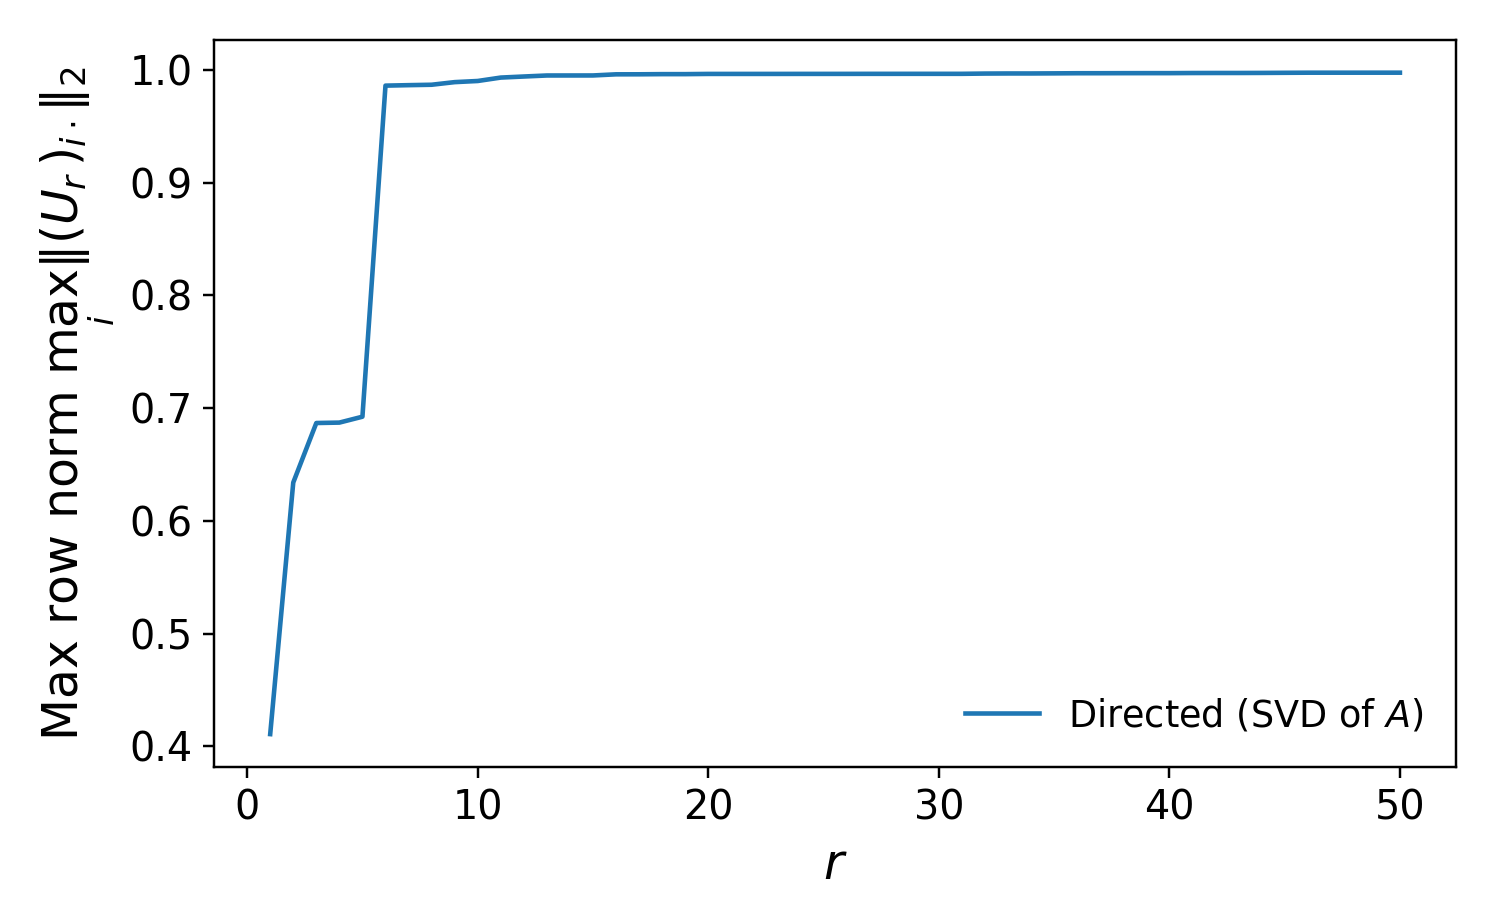
\includegraphics[width=0.92\linewidth]{figs/celegans_max_rownorm_directed.png}
  \vspace{-0.7em}
  \caption*{\footnotesize
  $\max_i \|(\mU_r)_{i\cdot}\|_2$ under different $r$ (SVD).}
\end{figure}
\end{column}

\end{columns}
\end{beamercolorbox}
}

\only<5>{
\vspace{-4em}
\begin{itemize}
  \item \textbf{Is the dependence on $\mu$ optimal?}\\
  One would argue that the row-wise estimation error depends on the row norm, so the dependence is natural. 
\end{itemize}
}

% ---------- <6->: remove columns; show lower bound + takeaway ----------
\only<6->{
    \vspace{-4em}
    \begin{itemize}
      \item \textbf{Lower bound.}
      If $(W_{ij})_{1\le i\le j\le n} \stackrel{i.i.d.}{\sim} \mathcal N(0,\sigma^2)$,
      \[
        \inf_{\widehat{\mU}} \sup_{\mu(\mUstar)\le \mu}
        \E \min_{\mO\in\bbO_r}
        \|\widehat{\mU}\mO - \mUstar\|_{2,\infty}
        =
        \Omegatilde\!\left(
          \frac{\sigma}{\lambdastar_{\min}}
          \wedge
          \sqrt{\frac{\mu}{n}}
        \right),
        \hfill \text{\citep{yan2024coherence}}.
      \]
    \end{itemize}
    
    \vspace{0.25em}
    \only<7->{
    \begin{alertblock}{Takeaway}
    \small
    \begin{itemize}
      \item<7-> Spectral estimator is \emph{not} minimax-optimal: error scales with coherence $\mu$.
      \item<8-> \textbf{Goal:} use multiple observations to achieve optimality. 
      \[
        \min_{\boldsymbol{O}\in\mathbb{O}_r}
        \left\|
        \boldsymbol{U}\widehat{\boldsymbol{\Psi}}
        - \boldsymbol{U}^{\star}\boldsymbol{O}
        \right\|_{2,\infty}
        = \tilde{O}\!\left(\frac{\sigma}{\lambda_{\min}^{\star}}\right).
      \]
    \end{itemize}
    \end{alertblock}
    }
}

% Reserve space on <1–2> so later overlays don't shift
\only<1-2>{\vphantom{\rule{0pt}{0.54\textheight}}}

\end{overlayarea}

\end{frame}









% ------------------------------------------------------------------

% --------------------------------------------------------------------



\begin{frame}{Eigenvalue Estimation with Two Independent Copies}

% ===================== Top: full-width baseline =====================
\begin{itemize}
    \item \textbf{Setup (rank-one signal).}
    $\mM^\star=\lambdastar \vustar \vustart \in \R^{n\times n}$.

    \medskip
    \item \pause \textbf{Single noisy copy.}
    If $\mY=\mM^\star+\mW$, the spectral estimator $\lambda$ satisfies
    \[
        \left|\lambda - \lambdastar\right|
        \;\le\; \|\mW\|
        \;\lesssim\; \sigma \sqrt{n}.
    \]
\end{itemize}

\vspace{0.8em}

% ===================== Bottom: split for structural gain =====================
\pause
% ===================== Bottom: split for structural gain =====================
% (after the top part; keep your existing top itemize with pauses)
\begin{columns}[T,onlytextwidth]

% -------- Left: two-copy results --------
\begin{column}{0.58\textwidth}
\begin{itemize}
    % 3rd bullet: show on overlay 3 and stay visible afterwards
    \item<3-> \textbf{Two independent copies: structural gain.}
    With $\mY_1=\mM^\star+\mW_1$ and $\mY_2=\mM^\star+\mW_2$,
    form $\mM$ by \emph{asymmetric rearrangement} (right), yielding
    \[
        |\widehat{\lambda}-\lambdastar|
        \;\lesssim\; \sigma\sqrt{\mu\log n}
        \qquad \text{\citep{chen2021asymmetry}.}
    \]

    \medskip
    % 4th bullet: show on overlay 5 and stay visible afterwards
    \item<5-> \textbf{Refined analysis (moment method).}
    \[
    \begin{aligned}
        &|\widehat{\lambda}-\lambdastar|
        \;\lesssim\;
        \max\!\left\{
            \frac{L\,\mu \log^5 n}{n},
            \;\sigma \log^{7/2} n
        \right\}
        \\ 
        &\text{\citep{yan2025improved}.}
    \end{aligned}
    \]
\end{itemize}
\end{column}

% -------- Right: visual panel --------
\begin{column}{0.4\textwidth}
\centering

% Figure appears on overlay 4 (and stays)
\only<4->{
\resizebox{0.6\linewidth}{!}{%
\begin{tikzpicture}[x=1.2cm,y=1.2cm]
  \def\n{4.8}

  % M =
  \node[anchor=east,font=\bfseries\Huge] at (-0.02*\n,0.5*\n) {$M=$};

  \fill[black!10] (0,\n) -- (\n,\n) -- (\n,0) -- cycle;
  \fill[black!25] (0,0) -- (0,\n) -- (\n,0) -- cycle;
  \draw[very thick] (0,0) rectangle (\n,\n);
  \draw[very thick] (0,\n) -- (\n,0);

  \node[font=\bfseries\Huge] at (0.68*\n,0.72*\n) {$Y_1$};
  \node[font=\bfseries\Huge] at (0.32*\n,0.28*\n) {$Y_2$};
  \node[font=\Large] at (0.78*\n,0.58*\n) {$i<j$};
  \node[font=\Large] at (0.22*\n,0.42*\n) {$i\ge j$};
\end{tikzpicture}%
}
\vspace{0.75em}
}

% Takeaway appears on overlay 6 (and stays)
\only<6->{
\begin{beamercolorbox}[rounded=true,shadow=true,wd=0.9\linewidth,sep=1.1ex]{block body alerted}
\small
\textbf{Key message.}
Two independent observations enable \emph{structural} improvements—beyond variance reduction.
\end{beamercolorbox}
}

\end{column}
\end{columns}

\end{frame}


\begin{frame}{Alternative Approaches to Use Two Independent Copies}

\begin{itemize}
    %\item \textbf{Context and motivation.}
    %\cite{fan2022asymptotic} use \emph{edge-splitting} to create independent graph copies for dimension estimation.
    %\cite{xie2024bias} propose a bias-corrected joint spectral embedding for multilayer networks.
    %\vspace{0.25em}
    \item \textbf{Alternative estimator for $\lambdastar$.}
    Motivated by the approach in \cite{fan2022asymptotic}, let $\vu_{\mathrm{sp}}$ denote the leading eigenvector estimated from $\mY_1$.
    Using an independent copy 
    $
        \mY_2 = \lambdastar \vustar\vustart + \mW_2,
    $
    \pause 
    \[
    \begin{aligned}
        \vu_{\mathrm{sp}}^\top \mY_2 \vu_{\mathrm{sp}}
        &=
        \lambdastar (\vustart \vu_{\mathrm{sp}})^2
        +
        \vu_{\mathrm{sp}}^\top \mW_2 \vu_{\mathrm{sp}}
        =
        \lambdastar (\vustart \vu_{\mathrm{sp}})^2
        +
        \widetilde O(\sigma) \\
        \pause 
        &= \lambdastar + O\left(\frac{\sigma^2 n}{\lambdastar}\right) + \widetilde O(\sigma)
    \end{aligned}
    \]

    \vspace{0.25em}

    \item \pause \textbf{Asymptotic correction.}
    Under homoscedastic noise, the BBP transition implies
    \[
        (\vustart \vu_{\mathrm{sp}})^2
        =
        1 - \frac{\sigma^2 n}{(\lambdastar)^2}
        + O_p(n^{-1}),
    \]
    \pause leading to \citep{chen2021asymmetry}
    \[
        \vu_{\mathrm{sp}}^\top \mY_2 \vu_{\mathrm{sp}}
        \approx \lambdastar
        - \frac{\sigma^2 n}{\lambdastar} \implies \lambdastar \approx \frac{\vu_{\mathrm{sp}}^\top \mY_2 \vu_{\mathrm{sp}}+\sqrt{(\vu_{\mathrm{sp}}^\top \mY_2 \vu_{\mathrm{sp}})^2+4 \sigma^2 n}}{2} 
    \]

    \pause 
    \begin{exampleblock}{Caveat}
    \begin{itemize}
        \item For the first approach, although it improves upon variance-reduction, it is not yet optimal. 
        \item \pause BBP-type bias correction becomes delicate in more general settings.
    \end{itemize}
    \end{exampleblock}
    
\end{itemize}

\end{frame}



\begin{frame}{Subspace Estimation: A Technical Tool}
\begin{itemize}
    \item \textbf{Setup.}
    Let $\mM$ denote the asymmetrically constructed matrix.
    For $l=1,\dots,r$, define the right eigenvectors by %and left eigenvectors by
    \[
        \mM \vu_l = \lambda_l \vu_l,
        %\qquad
        %\mM^\top \vw_l = \lambda_l \vw_l.
    \]
    Let $\mU := [\vu_1,\dots,\vu_r]$ denote the right eigenspace, $\mLambda = \operatorname{diag}(\lambda_1, \cdots, \lambda_r)$

    \item \pause \textbf{Key tool: Neumann expansion.}
    Writing $\mM = \mM^\star + \mH$, we obtain
    \[
    \begin{aligned}
        \vu_l
        &=
        \sum_{j=1}^r
        \frac{\lambda_j^\star}{\lambda_l}
        \left(\vustart_j \vu_l\right)\vustar_j
        +
        \sum_{j=1}^r
        \frac{\lambda_j^\star}{\lambda_l}
        \left(\vustart_j \vu_l\right)
        \Bigg\{
            \sum_{s=1}^\infty
            \frac{1}{\lambda_l^s}\mH^s\vustar_j
        \Bigg\}
        \\
        \pause &=
        \sum_{j=1}^r
        \frac{\lambda_j^\star}{\lambda_l}
        \left(\vustart_j \vu_l\right)\vustar_j
        \;+\;
        \widetilde{\mathcal{O}}\!\left(
            \frac{\sigma}{\lambda_{\min}^\star}
        \right),
        \hfill
        \text{\citep{yan2025improved}.}
    \end{aligned}
    \]

    \pause 
    \begin{block}{Matrix form}
        Collecting the eigenvectors yields
    \[
        \mU
        \approx
        \mU^\star
        \mLambdastar
        \mU^{\star\top}
        \mU
        \mLambda^{-1} =: \mUstar \mF, \quad \mF := \mLambdastar
        \mU^{\star\top}
        \mU
        \mLambda^{-1}
        %\;=\;
        %\mU^\star \mR \mSig \mGamma^\top + \mE,
    \]
    \end{block}
    %\item \pause \textbf{Matrix form.}
    %Collecting the eigenvectors yields
    %\[
    %    \mU
    %    =
    %    \mU^\star
    %    \mLambdastar
    %    \mU^{\star\top}
    %    \mU
    %    \mLambda^{-1}
    %    \;+\;
    %    \mE
    %    %\;=\;
    %    %\mU^\star \mR \mSig \mGamma^\top + \mE,
    %\]
    %where $\mE \in \R^{n\times r}$ captures higher-order noise effects.
    %For $i \in [n]$ and $\ell \in [r]$,
    %%\[
     %   E_{i\ell}
     %%   =
       % \sum_{j=1}^r
       % \frac{\lambda_j^\star}{\lambda_\ell}
       % \left(\vustart_j \vu_\ell\right)
       % \sum_{s=1}^\infty
       % \frac{\ve_i^\top \mH^s \vustar_j}{\lambda_\ell^s}.
    %\]
\end{itemize}
\end{frame}



\begin{frame}{Subspace Estimation with More Copies}
\begin{itemize}
    \item \textbf{Matrix form.} %TODO: remind that this is from previous slide.
    \[
        \mU
        \approx
        \mU^\star
        \mLambdastar
        \mU^{\star\top}
        \mU
        \mLambda^{-1}
        \;=\;
        \mUstar \mF 
    \] %TODO make the connection with the last bullet point on previous slide more clear/explicit.
    \item The deviation from $\mU^\star$ is captured by the
multiplicative factor
$\mF$.
    \begin{itemize}
        \pause
        \item To recover $\mU^\star$ accurately, we must correct $\mU$ for the
    systematic distortion
        \pause
        \item Direct correction requires knowing $\mU^{\star\top}
        \mU$ accurately, which is challenging. 
    \end{itemize}
    \item \pause Singular value decomposition
    $$
    \mF := \mR \boldsymbol{\Sigma} \mGamma^\top
    $$
    \item \pause If $(\mF^\top \mF)^{-1/2} = \mGamma \boldsymbol{\Sigma}^{-1} \mGamma^\top$ is known, then 
    $$
    \mU \mGamma \boldsymbol{\Sigma}^{-1} \mGamma^\top \approx \mUstar \mR\boldsymbol{\Sigma} \mGamma^\top \mGamma \boldsymbol{\Sigma}^{-1} \mGamma^\top = \mUstar \mR \mGamma^\top. 
    $$
    %\item If additional independent samples are available, the eigenspace can be estimated more accurately under weaker eigengap conditions. 
    %Split this into two slides
    \item \pause \textbf{Goal:} Estimate $\mGamma \boldsymbol{\Sigma}^{-1} \mGamma^\top$ with additional copies. 
\end{itemize}
\end{frame}

\begin{frame}{Subspace Estimation with More Copies}
\begin{itemize}
    \item[] 
    \hspace{0.03\linewidth}
    \begin{beamercolorbox}[rounded=true,shadow=true,wd=0.9\linewidth,sep=0.4ex]{block body alerted}
    \textbf{First order approximation} %TODO: remind that this is from previous slide.
    $$
        \mU
        \approx
        \mU^\star
        \mLambdastar
        \mU^{\star\top}
        \mU
        \mLambda^{-1}
        \;=\; \mUstar \mF = 
        \mU^\star \mR \mSig \mGamma^\top.
    $$ %TODO make the connection with the last bullet point on previous slide more clear/explicit.
    \textbf{Goal:} Estimate $(\mF^\top \mF)^{-1/2} = \mGamma \boldsymbol{\Sigma}^{-1} \mGamma^\top$. 
    \end{beamercolorbox}
    \item Suppose that we observe two extra independent copies, $\boldsymbol{Y}^{(1)}$ and $\boldsymbol{Y}^{(2)}$, each generated as
$$
\boldsymbol{Y}^{(i)}=\boldsymbol{M}^{\star}+\boldsymbol{W}_i, \quad \text { for } i=1,2 .
$$ %TODO: make sure you remind everyone that this is two MORE indep copies, so now we have four in total.
\item \pause Define the matrix %TODO: point out that U, Lambda are coming from the first two matrices, and we are using two more to refine the estimate.
\vspace{-0.8em}
\begin{equation*}
    \boldsymbol{G}:=\left(\boldsymbol{\Lambda}^{-1} \boldsymbol{U}^{\top} \boldsymbol{Y}^{(1)} \boldsymbol{Y}^{(2)} \boldsymbol{U} \boldsymbol{\Lambda}^{-1}\right)^{-1} \pause \approx \left(\underbrace{\boldsymbol{\Lambda}^{-1} \boldsymbol{U}^{\top} \mUstar \mLambdastar}_{\mF^\top} \underbrace{\mLambdastar\mUstart \boldsymbol{U} \boldsymbol{\Lambda}^{-1}}_{\mF}\right)^{-1}
\end{equation*}
%\pause and its symmetrized version 
%$
%\boldsymbol{G}_{\mathrm{symm}}:=\frac{1}{2}\left(\boldsymbol{G}+\boldsymbol{G}^{\top}\right) .
%$
\vspace{-0.4em}
\item \pause Let $\widehat{\boldsymbol{\Psi}} := \left[\frac{1}{2}(\mG+ \mG^\top)\right]^{1/2}$, \cite{yan2025estimating} shows that 
$$
\min _{\boldsymbol{O} \in \mathbb{O}_r}\left\|\boldsymbol{U} \widehat{\boldsymbol{\Psi}}-\boldsymbol{U}^{\star} \boldsymbol{O}\right\|_{2, \infty} = \tilde{O}\left(\frac{\sigma}{\lambda_{\min }^{\star}}\right)
$$
\end{itemize}
\end{frame}


%\begin{frame}{Method: Step II}
%\begin{itemize}
    
%    \pause
%    \item Observation II: If both $\lambdastar > 0$ and $\vustar \geq 0$, then  
    
%\end{itemize}
%\end{frame}

\begin{frame}{Experiment Setup}

\textbf{Data generation.}
\begin{itemize}
    \item Four matrices $\mY_{11}, \mY_{12}, \mY_{21}, \mY_{22}$ are generated from a low-rank-plus-noise model
    with rank $r=3$ and i.i.d.\ standard normal noise.
    \pause
    \item Matrix dimension $n$ varies from $700$ to $40{,}000$.
    \pause
    \item Incoherence parameter $\mu \in \{n^{4/5},\, n^{5/6}\}$.
    \pause
    \item Minimum nonzero eigenvalue of $\mM^\star$ is
    $\lambdastar_{\min} = 2.05 \sqrt{n}$.
    \pause
    \item Eigengaps are set to be $\log n$. 
    \pause
    \item For each $i=1,2$, construct $\mM_i$ by asymmetrically arranging $\mY_{i1}$ and $\mY_{i2}$.
\end{itemize}

\pause
\textbf{Estimators.}
\begin{itemize}
    \item \textbf{(i) Naive spectral averaging:}
    Average all four matrices $\mY_{ij}$ and compute the spectral estimator
    $\widehat{\mU}_{\mathrm{sp}}$
    \item \pause \textbf{(ii) Single-pair debiased:}
    Apply the bias-corrected eigenspace estimator $\widehat{\mU}$ to
    the averaged asymmetric matrix $\mM_{\mathrm{asym}}$ formed from $\mM_1$ and $\mM_2$ %and set
    %$
    %    \widehat{\mM} := \widehat{\mU}\,\mLambda\,\widehat{\mU}^\top .
    %$
    \item \pause \textbf{(iii) Refined debiased:}
    Use the refined eigenspace estimator $\mU \mPsihat$ %and the final estimator
    %$\widehat{\mM}_{\mathrm{de}}$.
\end{itemize}

\end{frame}


\begin{frame}{Numerical Results: Subspace Estimation}
\begin{figure}[t]
    \centering
    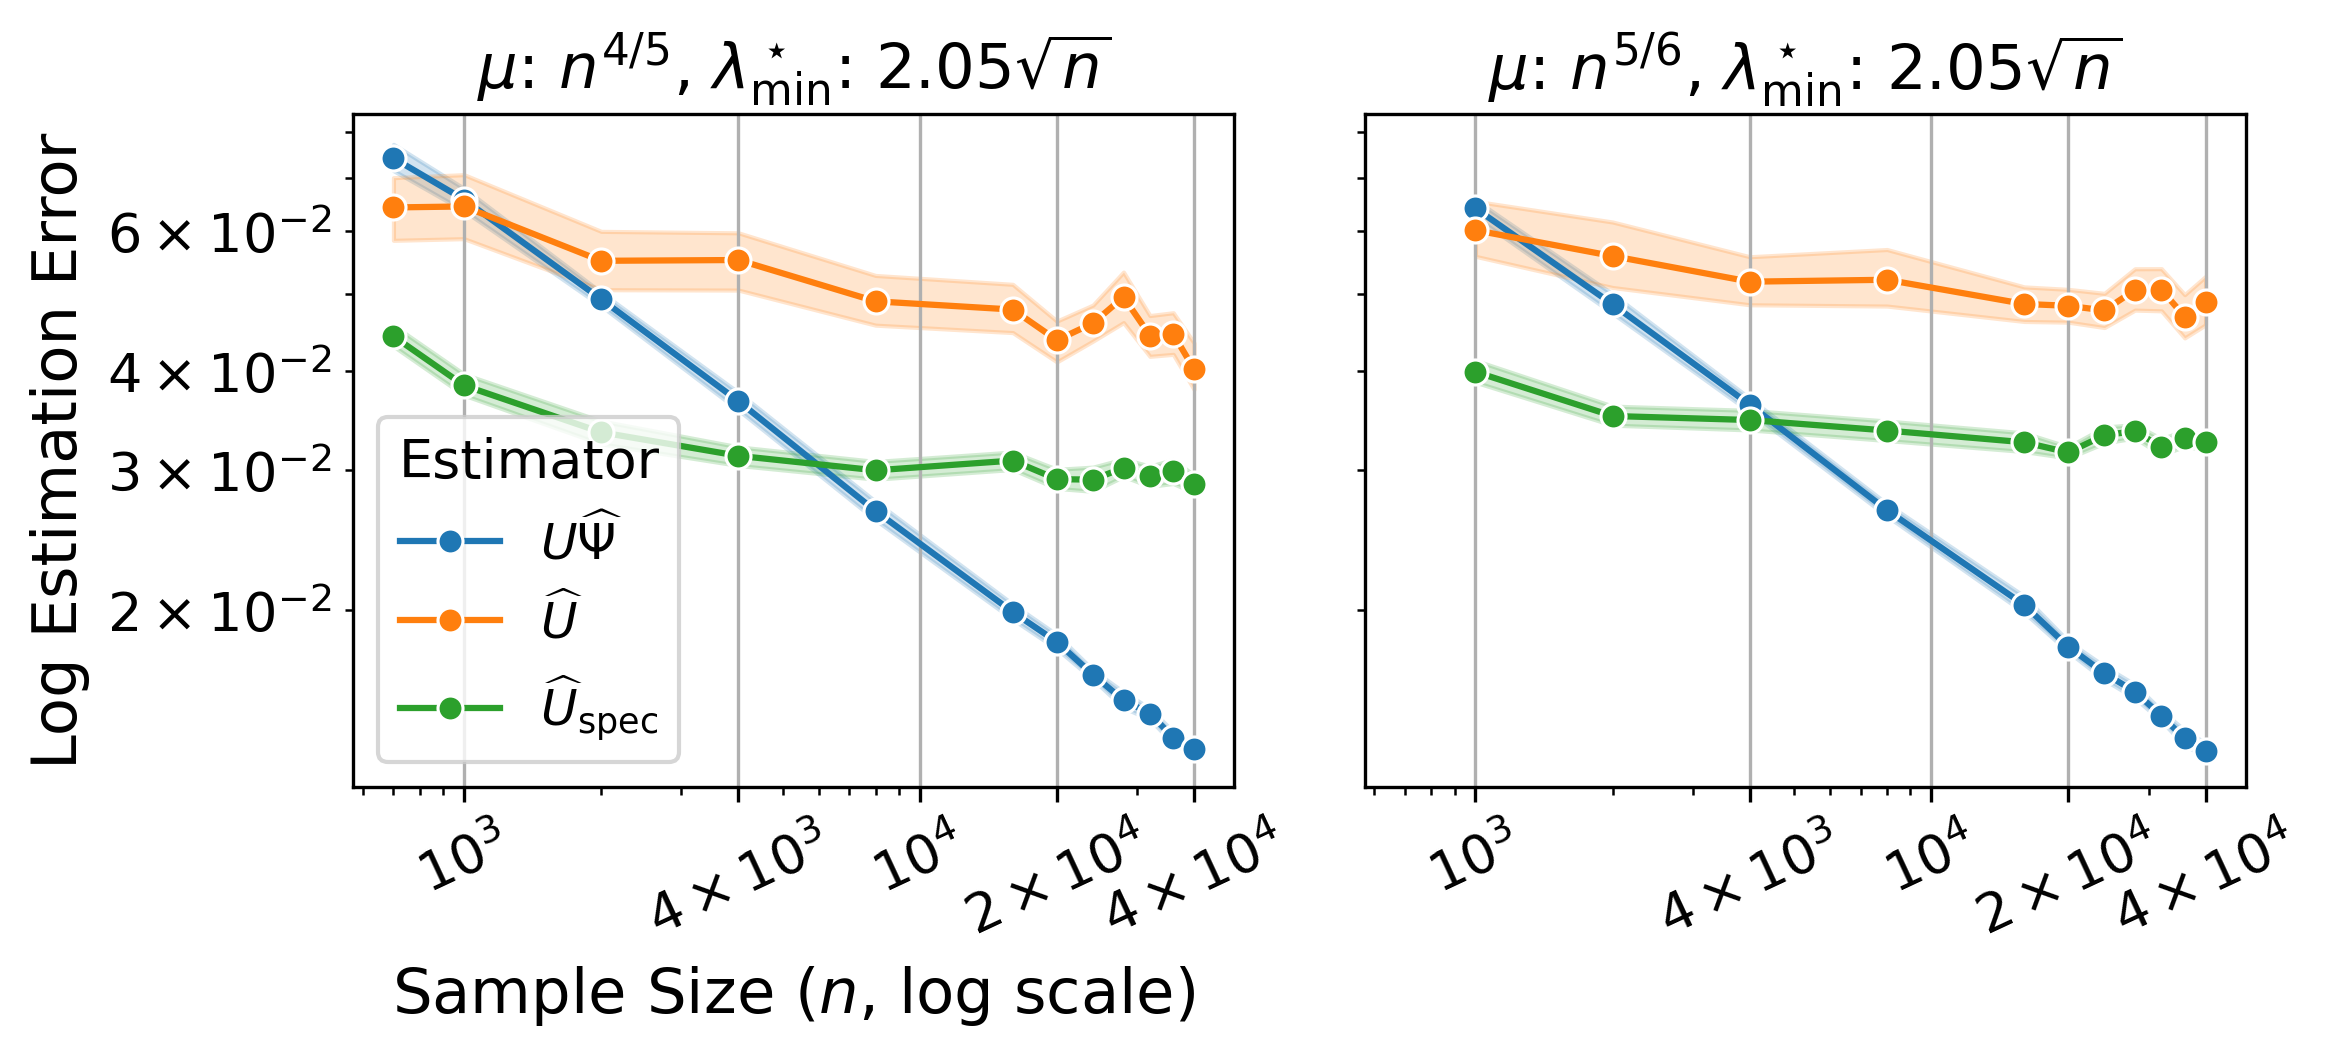
\includegraphics[width=0.8\textwidth]{figs/exp5plotU_split_lam0.png}
\end{figure}
\begin{itemize}
    \item The $y$-axis reports the log estimation error in the $(2,\infty)$-norm.
    %\item Among the three methods, $\widehat{\mU}$ exhibits the largest error,
    %dominated by a $\sqrt{\mu/n}/\deltastar_{\min}$ term that decays slowly with $n$.
    \pause
    \item The spectral estimator $\widehat{\mU}_{\mathrm{sp}}$ is driven by
    $\sqrt{\mu}/\lambdastar_{\min}$.
    As $n$ grows, its error plateaus and eventually exceeds that of the refined estimator
    $\mU \mPsihat$.
\end{itemize}
\end{frame}

%\begin{frame}{Other Estimation Targets}

%\begin{itemize}
%    \item \textbf{Linear functionals of eigenvectors} \; For fixed \(\va\) with \(\|\va\|_2=1\):
%        $$
%        \left| \va^\top \widehat{\vu}_\ell - \va^\top \vu^\star_\ell \right|
%        $$
%    \pause 
%    \item \textbf{Entrywise eigenvector estimation}
%        $$
%        \min \left\|\widehat{\vu}_\ell \pm \vu^\star_\ell\right\|_\infty
%        $$
%    \pause 
%    \item \textbf{Entrywise low-rank matrix estimation}
%        $$
%        \left\|\widehat{\mM}-\mM^\star\right\|_{\infty} := \max_{i,j} \left|\widehat{M}_{ij}-M^\star_{ij}\right|
%        $$
    

    %\item \pause \textbf{Eigenspace / subspace estimation}
    %    $$
    %    \min_{\mO\in\mathbb{O}(r)} \|\widehat{\mU}\mO-\mU^\star\|_{2,\infty}
    %    $$
    
%\end{itemize}

%\end{frame}

%\begin{frame}{Other Estimates of Interest}
    
%\end{frame}

% Preamble:
% \usepackage{tikz}
% \usetikzlibrary{calc}

\begin{frame}{Beyond Identical Replications: Sparse Differences Between Groups}
\small

% Freeze overall body height (prevents global reflow across overlays)
\begin{overlayarea}{\textwidth}{0.86\textheight}

\begin{itemize}
    \item<1-> \textbf{Motivation.}
    Multiple replications are idealized; in practice different groups may exhibit \emph{structured} variation.

    \item<2-> \textbf{Structured difference.}
    $\mB^\star$ is symmetric and decomposes as $\mB^\star=\mB_0+\mB_0^\top$,
    where $\mB_0$ is \textbf{row-sparse}.
    \emph{Goal: recover the support of $\mB_0$.}

    % Fixed-height columns block appears starting at <2>, but its space is reserved so later items don't move.
    \item[]<2->%
    \begin{overlayarea}{\textwidth}{0.52\textheight} % tune once; then stable
    \begin{columns}[T,onlytextwidth]

    % ---------------- Left column ----------------
    \begin{column}{0.60\textwidth}

        \vspace{0.25em}
        \hspace*{0.1\linewidth}
        \begin{beamercolorbox}[rounded=true,shadow=true,wd=0.6\linewidth,sep=1.0ex]{block body}
        \[
            \mY^{(0)} = \mM^\star + \mW^{(0)}
        \]
        \[
            \mY^{(1)} = \mM^\star + \mB^\star + \mW^{(1)} .
        \]
        \end{beamercolorbox}

        \vspace{0.35em}

        % Swap region: fixed height so nothing shifts when figure is replaced by text
        \begin{overlayarea}{\linewidth}{0.33\textheight} % tune to match figure footprint
            \only<3>{
            \begin{figure}
                \centering
                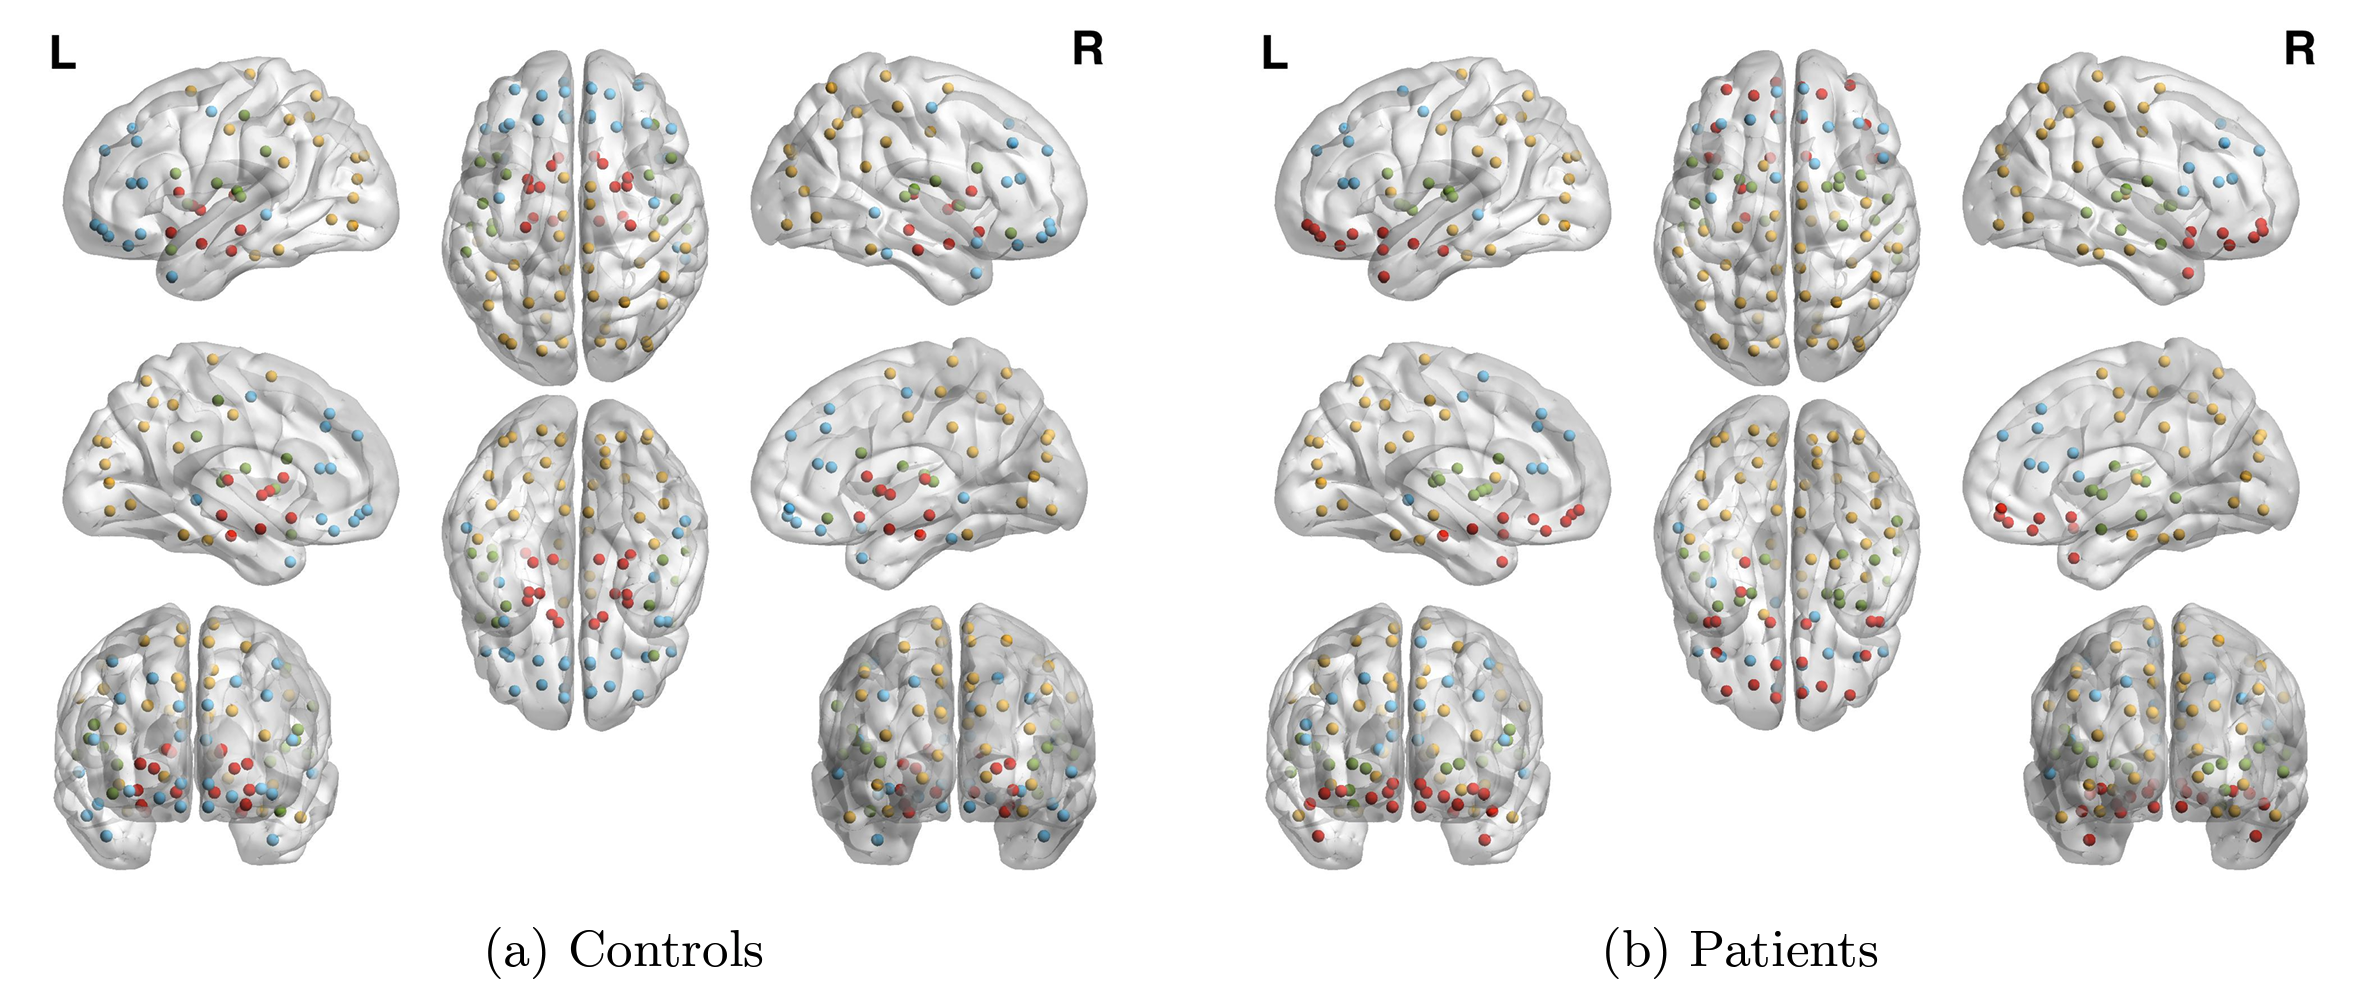
\includegraphics[width=\linewidth]{figs/brains.png}
            \end{figure}
            }
            \only<4->{
            \begin{itemize}
                \item \textbf{Two-step estimator.}
                \begin{enumerate}
                    \item Form a spectral estimator $\widehat{\mM}_{\mathrm{sp}}$ from $\mY^{(0)}$.
                    \item Use the residual
                    \[
                        \mY^{(1)} - \widehat{\mM}_{\mathrm{sp}}
                        = \mB^\star + (\mM^\star-\widehat{\mM}_{\mathrm{sp}}) + \mW^{(1)}
                    \]
                    to estimate the support.
                \end{enumerate}
            \end{itemize}
            }
        \end{overlayarea}

    \end{column}

    % ---------------- Right column ----------------
    \begin{column}{0.38\textwidth}
        \centering
        \begin{beamercolorbox}[rounded=true,shadow=true,wd=0.8\linewidth,sep=0.8ex]{block body}
        \centering
        \resizebox{0.7\linewidth}{!}{%
        \begin{tikzpicture}[x=0.35cm,y=0.35cm]
          \def\n{10}
        
          % Background
          \fill[black!6] (0,0) rectangle (\n,\n);
          \draw[very thick] (0,0) rectangle (\n,\n);
        
          % Row blocks (row index increases downward)
          \foreach \r in {3,7} {
            \fill[black!35] 
              (0,\n-\r) rectangle (\n,\n-\r+1);
          }
        
          % Column blocks (column index increases rightward)
          \foreach \c in {3,7} {
            \fill[black!35] 
              (\c-1,0) rectangle (\c,\n);
          }
        
          % Title
          \node[font=\bfseries\Large] 
            at (0.5*\n,1.12*\n) {$\mathrm{supp}(\mB^\star)$};
        \end{tikzpicture}
        }
        \end{beamercolorbox}
    \end{column}

    \end{columns}
    \end{overlayarea}

    \vspace{-2.5em}  % adjust to taste
    
    \item<5-> An SDP-based support recovery method achieves minimax-optimal rates (under suitable conditions),

    \item<6-> There is a \textbf{fundamental gap} between single-copy vs multi-copy access for recovering $\mathrm{supp}(\mB^\star)$.
\end{itemize}

\end{overlayarea}
\end{frame}






\begin{frame}{Summary}

\begin{itemize}
    \item \textbf{Problem.}
    Recover a shared low-rank signal from multiple independent noisy observations
    on the same set of nodes.
    \pause
    \item \textbf{Key insight.}
    Simple averaging offers trivial benefit for global losses,
    but multiple observations \textbf{dramatically improve} fine-grained recovery.
    \pause
    \item \textbf{Methodology.}
    We introduce debiased and refined spectral estimators that exploit asymmetry across observations
    to mitigate bias induced by high coherence.
    \pause
    \item \textbf{Theory.}
    Additional copies enable minimax-optimal rates for eigenspace.
    \pause
    \item \textbf{Empirical evidence.}
    Simulations validate the theory. %and suggest that some apparent theoretical dependencies
    %(e.g., eigenvalue spread) are artifacts rather than fundamental limits.
    
    \pause 
    
    \medskip
    \centering
    \emph{Multiple observations unlock stronger network recovery.}
    \medskip
    \begin{center}
        \large Thank you!
    \end{center}
    \medskip
    \begin{center}
    \begin{minipage}{10cm}
    \footnotesize{\textbf{Acknowledgement:} 
    Supported by NSF DMS 2052918, NSF DMS 2023239, and the University of Wisconsin-Madison Office of the Vice Chancellor for Research and Graduate Education with funding from the Wisconsin Alumni Research Foundation.}
    \end{minipage}
    \end{center}
\end{itemize}

\end{frame}

\appendix

\begin{frame}[allowframebreaks]{References}
\vspace{5mm}
\bibliographystyle{apalike}
\bibliography{bib}
\end{frame}



\begin{frame}{Noise Distributional Assumption}

Let $\mW \in \mathbb{R}^{n\times n}$ denote the noise matrix.

\medskip

\textbf{Assumption 1.}
The matrix $\mW$ is symmetric, with independent entries
$\{W_{ij}\}_{1\le i\le j\le n}$ on and above the diagonal.
Moreover, for all $1\le i\le j\le n$:

\begin{itemize}
    \item \pause \textbf{(Heteroscedastic variance)} 
    \[
        \mathbb{E}[W_{ij}^2]
        \;=\;
        \sigma_{ij}^2
        \;\le\;
        \sigma^2.
    \]

    \item \pause \textbf{(Boundedness)} 
    \[
        |W_{ij}| \;\le\; L,
        \; \text{with high probability, where } \sigma \leq L \ll \sigma \min \left\{\frac{n}{\mu \log^3 n}, \sqrt{\frac{n}{\log^3 n}}\right\}
    \]

    \item \pause \textbf{(Symmetry about zero)} 
    \[
        W_{ij} \;\overset{d}{=}\; -W_{ij}.
    \]
\end{itemize}

\pause

\begin{block}{Remark}
\begin{itemize}
    \item The first two conditions resembles the Bernstein moment condition. 
    \item The bound on $L$ is for presenting coherence-free results. 
    \item Symmetry requirement is a technical condition. 
\end{itemize}
\end{block}

\end{frame}


\begin{frame}{Rank Selection}
\begin{itemize}
    \item Construct a low-rank signal
    $
\mMstar,
$ with rank $r = 10$,
where $$\lambdastar_i=1.05 \sqrt{n}+(i-1) \cdot \mathrm{gap}.$$
\item Observe $\mM = \mMstar + \mH$, where $\mH$ has i.i.d. $
H_{i j} \sim \mathcal{N}(0,1).
$
\end{itemize}
\pause
\begin{figure}[htbp]
    \centering
    \begin{subfigure}{0.48\linewidth}
        \centering
        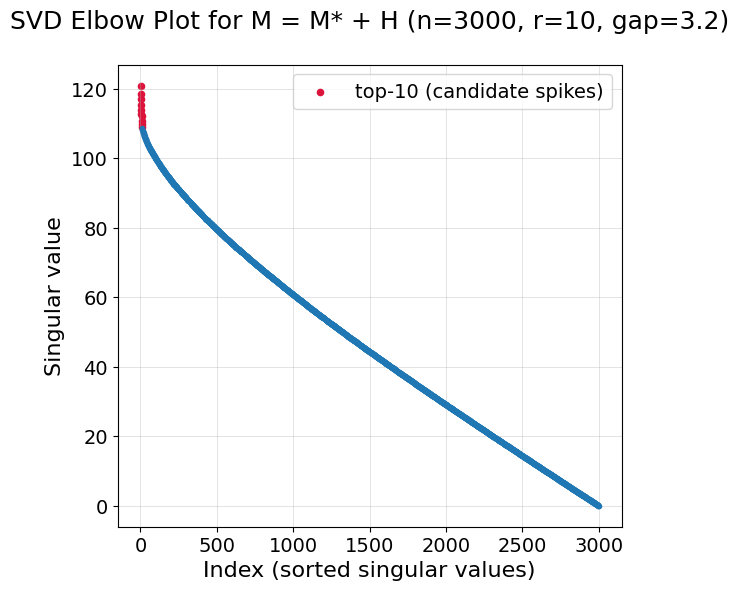
\includegraphics[width=\linewidth]{svd.png}
    \end{subfigure}\hfill
    \pause
    \begin{subfigure}{0.48\linewidth}
        \centering
        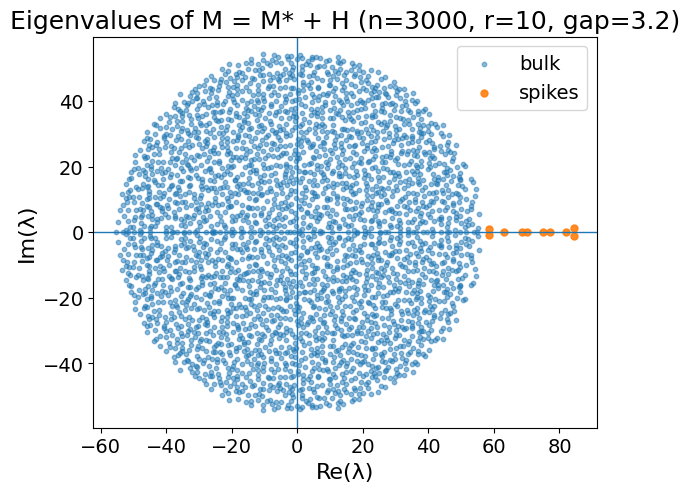
\includegraphics[width=\linewidth]{eigen.png}
    \end{subfigure}
\end{figure}

\end{frame}

\begin{frame}{Minimax Limits: Row-wise vs.\ Entrywise}

\begin{itemize}
    %\item \textbf{Coherence (eigenspace localization).}
    %For $\mM^\star = \mU^\star \mLambda^\star (\mU^\star)^\top$ with
    %$\mU^\star\in\mathbb{R}^{n\times r}$ orthonormal, define
    %\[
    %    \mu
    %    \;:=\;
    %    \frac{n}{r}\,\|\mU^\star\|_{2,\infty}^2
    %    \;=\;
    %    \frac{n}{r}\,\max_{i\in[n]} \|\mU^\star_{i,\cdot}\|_2^2,
    %    \qquad
    %    1 \le \mu \le \frac{n}{r}.
    %\]

    \item \textbf{Minimax lower bounds.}
    \begin{itemize}
        \item \textbf{Row-wise error \(\|\cdot\|_{2,\infty}\):}
        with $N\ge1$ independent observations,
        \[
            \inf_{\widehat{\mM}}
            \sup_{\mM^\star\in \mathcal{M}_0(\mu,\sigma_{\min})}
            \mathbb{E}\|\widehat{\mM}-\mM^\star\|_{2,\infty}
            \;\gtrsim\;
            \sigma_{\min}\sqrt{\frac{\mu}{N}}.
        \]

        \item \textbf{Entrywise error \(\|\cdot\|_{\infty}\):}
        for the rank-one class $\mathcal{M}(\mu,\sigma_{\min})$,
        \[
            \inf_{\widehat{\mM}}
            \sup_{\mM^\star\in \mathcal{M}(\mu,\sigma_{\min})}
            \mathbb{E}\|\widehat{\mM}-\mM^\star\|_{\infty}
            \;\gtrsim\;
            \frac{\sigma_{\min}}{\sqrt{N}}\sqrt{\frac{\mu}{n}}.
        \]
    \end{itemize}

    \item \textbf{Recall: spectral upper bounds}
    Using $\max_i \|\mU^\star_{i,\cdot}\|_2 \le \sqrt{\mu r/n}$:
    \begin{itemize}
        \item \textbf{Row-wise (upper):}
        \[
            \|\mDelta\|_{2,\infty}
            \;\lesssim\;
            \sigma\sqrt{\mu r}
            \;+\;
            \sigma\sqrt{r\log n}.
        \]

        \item \textbf{Entrywise (upper):}
        \[
            \|\mDelta\|_{\infty}
            \;\lesssim\;
            \sigma\,\frac{\mu r}{\sqrt{n}}
            \;+\;
            \sigma\,r\sqrt{\frac{\mu\log n}{n}}.
        \]
    \end{itemize}
    \begin{itemize}
        \item \textbf{Row-wise:} spectral estimator is rate-optimal (up to logs) for $N=\Theta(1)$.
        \item \textbf{Entrywise:} spectral estimator is \emph{not} minimax-optimal; error scales with
        coherence $\mu$, motivating bias correction and multiple observations.
    \end{itemize}
\end{itemize}

\end{frame}


\begin{frame}{Precise Bound on the Refined Estimator}
Under suitable noise assumptions and conditions on $\lambdastar_{\min}$ and $\deltastar_{\min}$,   
\begin{equation*}
    \min_{\mO \in \bbO_r} \left\|\mU \mPsihat - \mUstar \mO \right\|_{2, \infty} \lesssim \frac{\sigma \kappa r \sqrt{\log^7 n}}{\lambdastar_{\min}}
\end{equation*}
\end{frame}

\begin{frame}{Matrix Estimation with More Copies}
\begin{itemize}
    \item For entrywise estimation of $\mMstar$, we use 
    $$
    \widehat{\mM}_{\mathrm{de}} := \mU \widehat{\mPsi} \mLambda \widehat{\mPsi}^\top \mU^\top, 
    $$
    which satisfies
    $$
    \|\widehat{\mM}_{\mathrm{de}} - \mMstar\|_{\infty} = \tilde{O}\left(\sigma \sqrt{\frac{\mu}{n}} + \sigma \frac{\mu}{n} \frac{\deltastar_{\max}}{\deltastar_{\min}}\right),
    $$
    the dependence on the ratio between the eigengaps is most likely a technical artifact. 
    \item Recall that 
    $$
    \|\widehat{\mM}_{\mathrm{sp}} - \mMstar\|_{\infty} = \tilde{O}\left(\sigma \frac{\mu}{\sqrt{n}}\right)
    $$
    $\widehat{\mM}_{\mathrm{de}}$ improves upon the spectral estimator. 
    \item When $\frac{\deltastar_{\max}}{\deltastar_{\min}} \asymp \sqrt{\frac{n}{\mu}}$, $\widehat{\mM}_{\mathrm{de}}$ is near-minimax optimal.    
\end{itemize}
\end{frame}


\begin{frame}{Numerical Results: Incoherence Setting}
    \begin{figure}
        \centering
        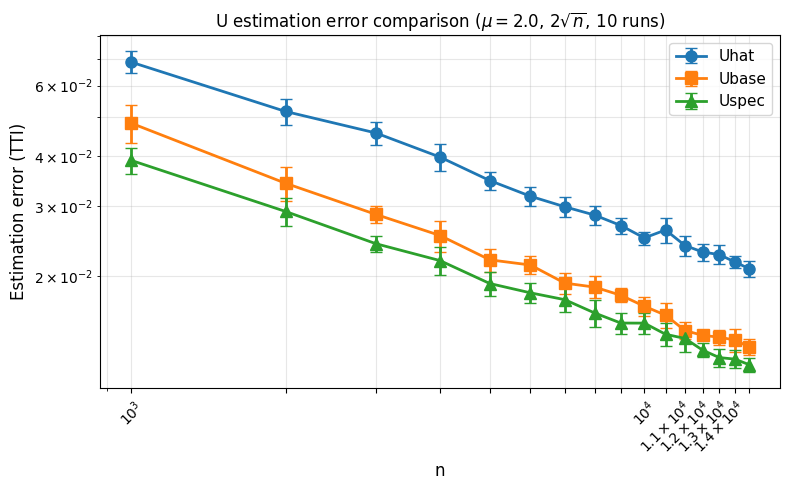
\includegraphics[width=0.75\linewidth]{incoherent.png}
    \end{figure}
\end{frame}

\begin{frame}{Numerical Results: Entrywise Estimation}
\begin{figure}[t]
    \centering
    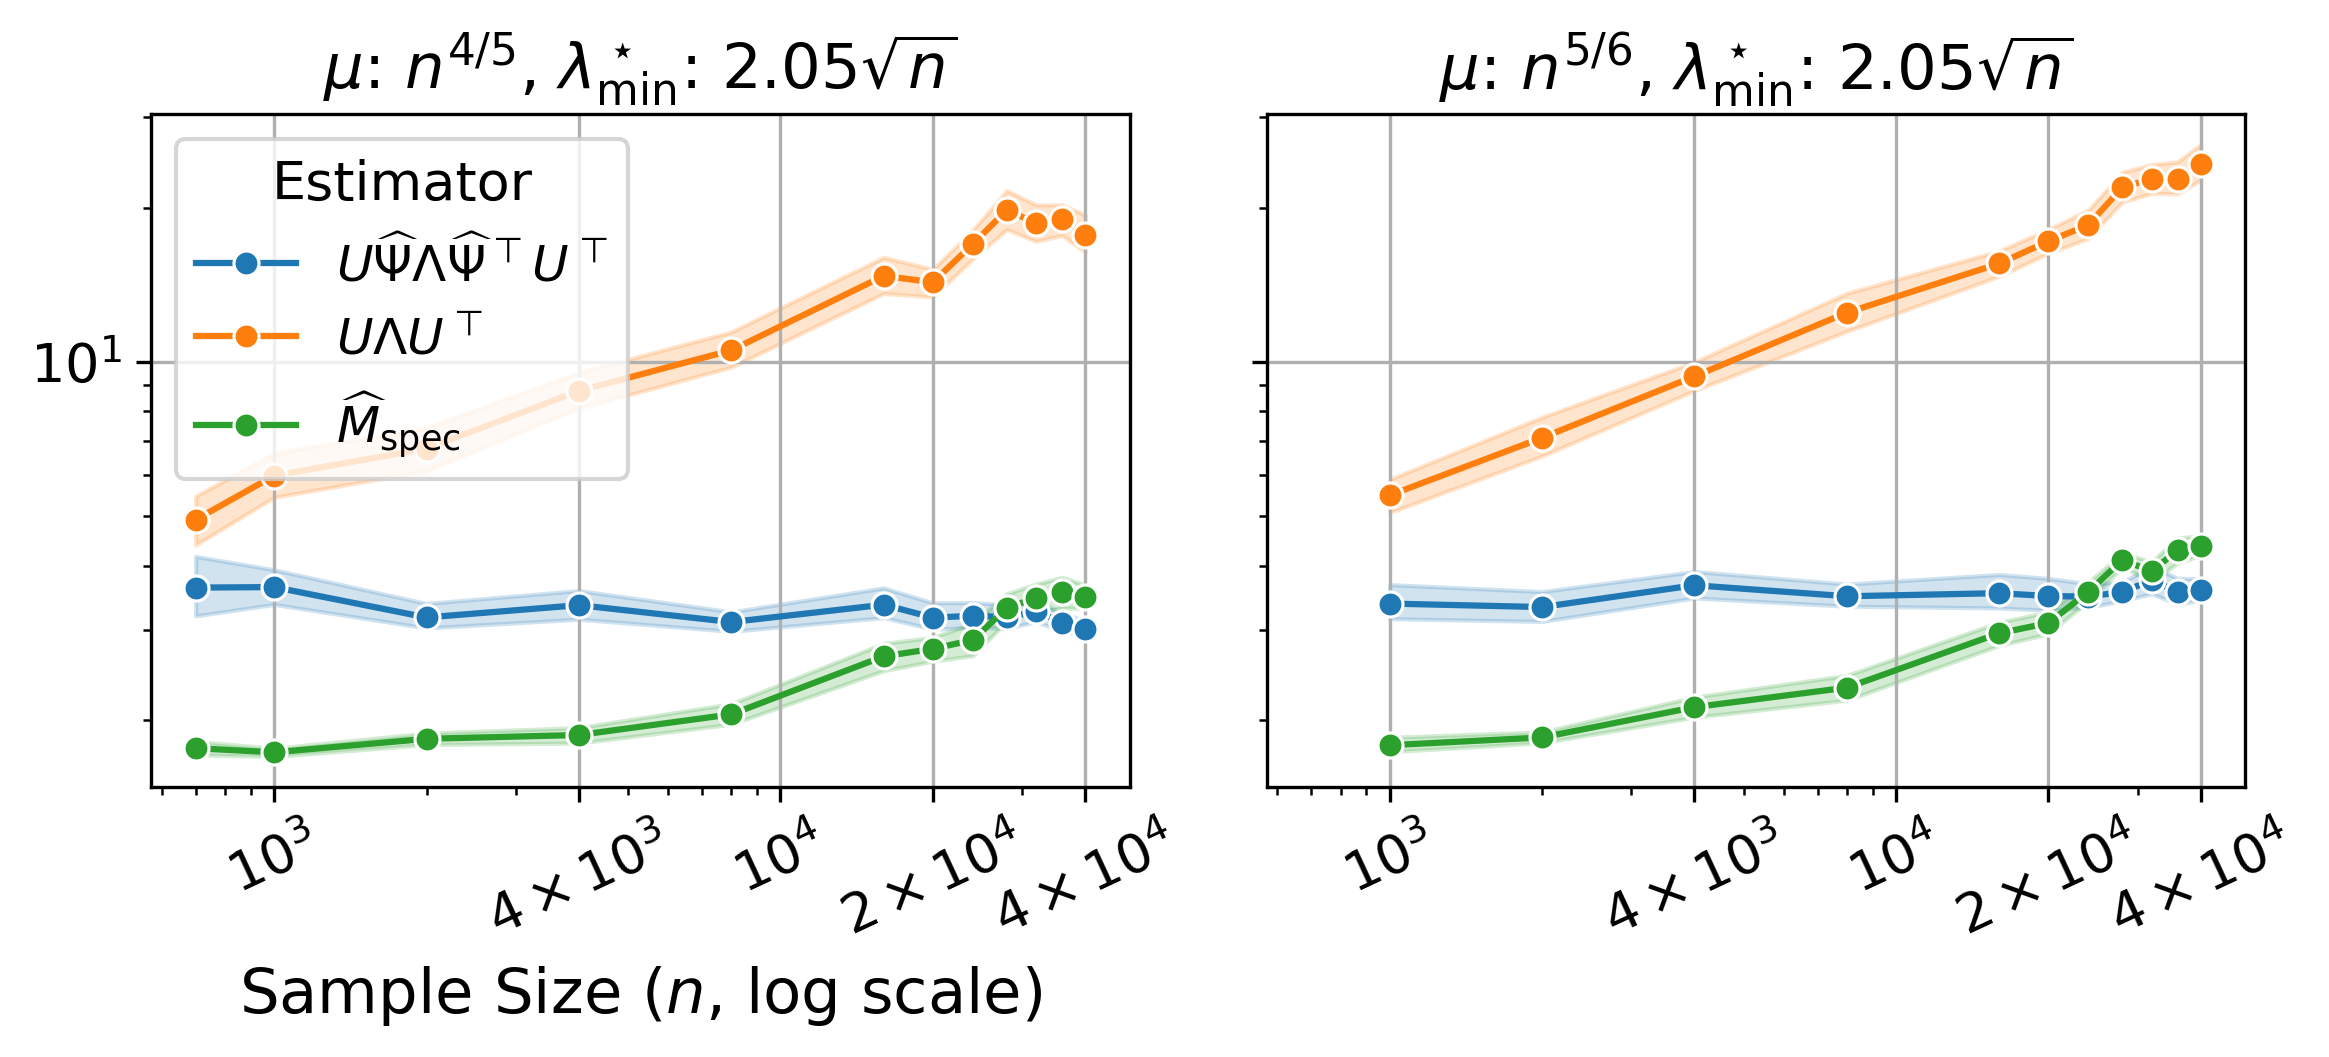
\includegraphics[width=0.8\textwidth]{figs/exp5plotM_split_lam0.png}
\end{figure}
\begin{itemize}
    \item The $y$-axis reports the log estimation error in the $\infty$-norm.
    \item Among the three methods, $\widehat{\mU} \mLambda \widehat{\mU}$ exhibits the largest error,
    dominated by a $\lambdastar_{\max}/\deltastar_{\min} \cdot \mu/n$ term that increases in $n$.
    \item The spectral estimator $\widehat{\mM}_{\mathrm{sp}}$ is driven by
    $\mu/\sqrt{n}$.
    As $n$ grows, its error plateaus and eventually exceeds that of the refined estimator
    $\widehat{\mM}_{\mathrm{de}}$.
\end{itemize}
\end{frame}


\begin{frame}{Numerical Results: Varying Eigengap Ratio}
%Previous analysis shows that when $\rho = \sqrt{n / \mu}$  
\begin{figure}
    \centering
    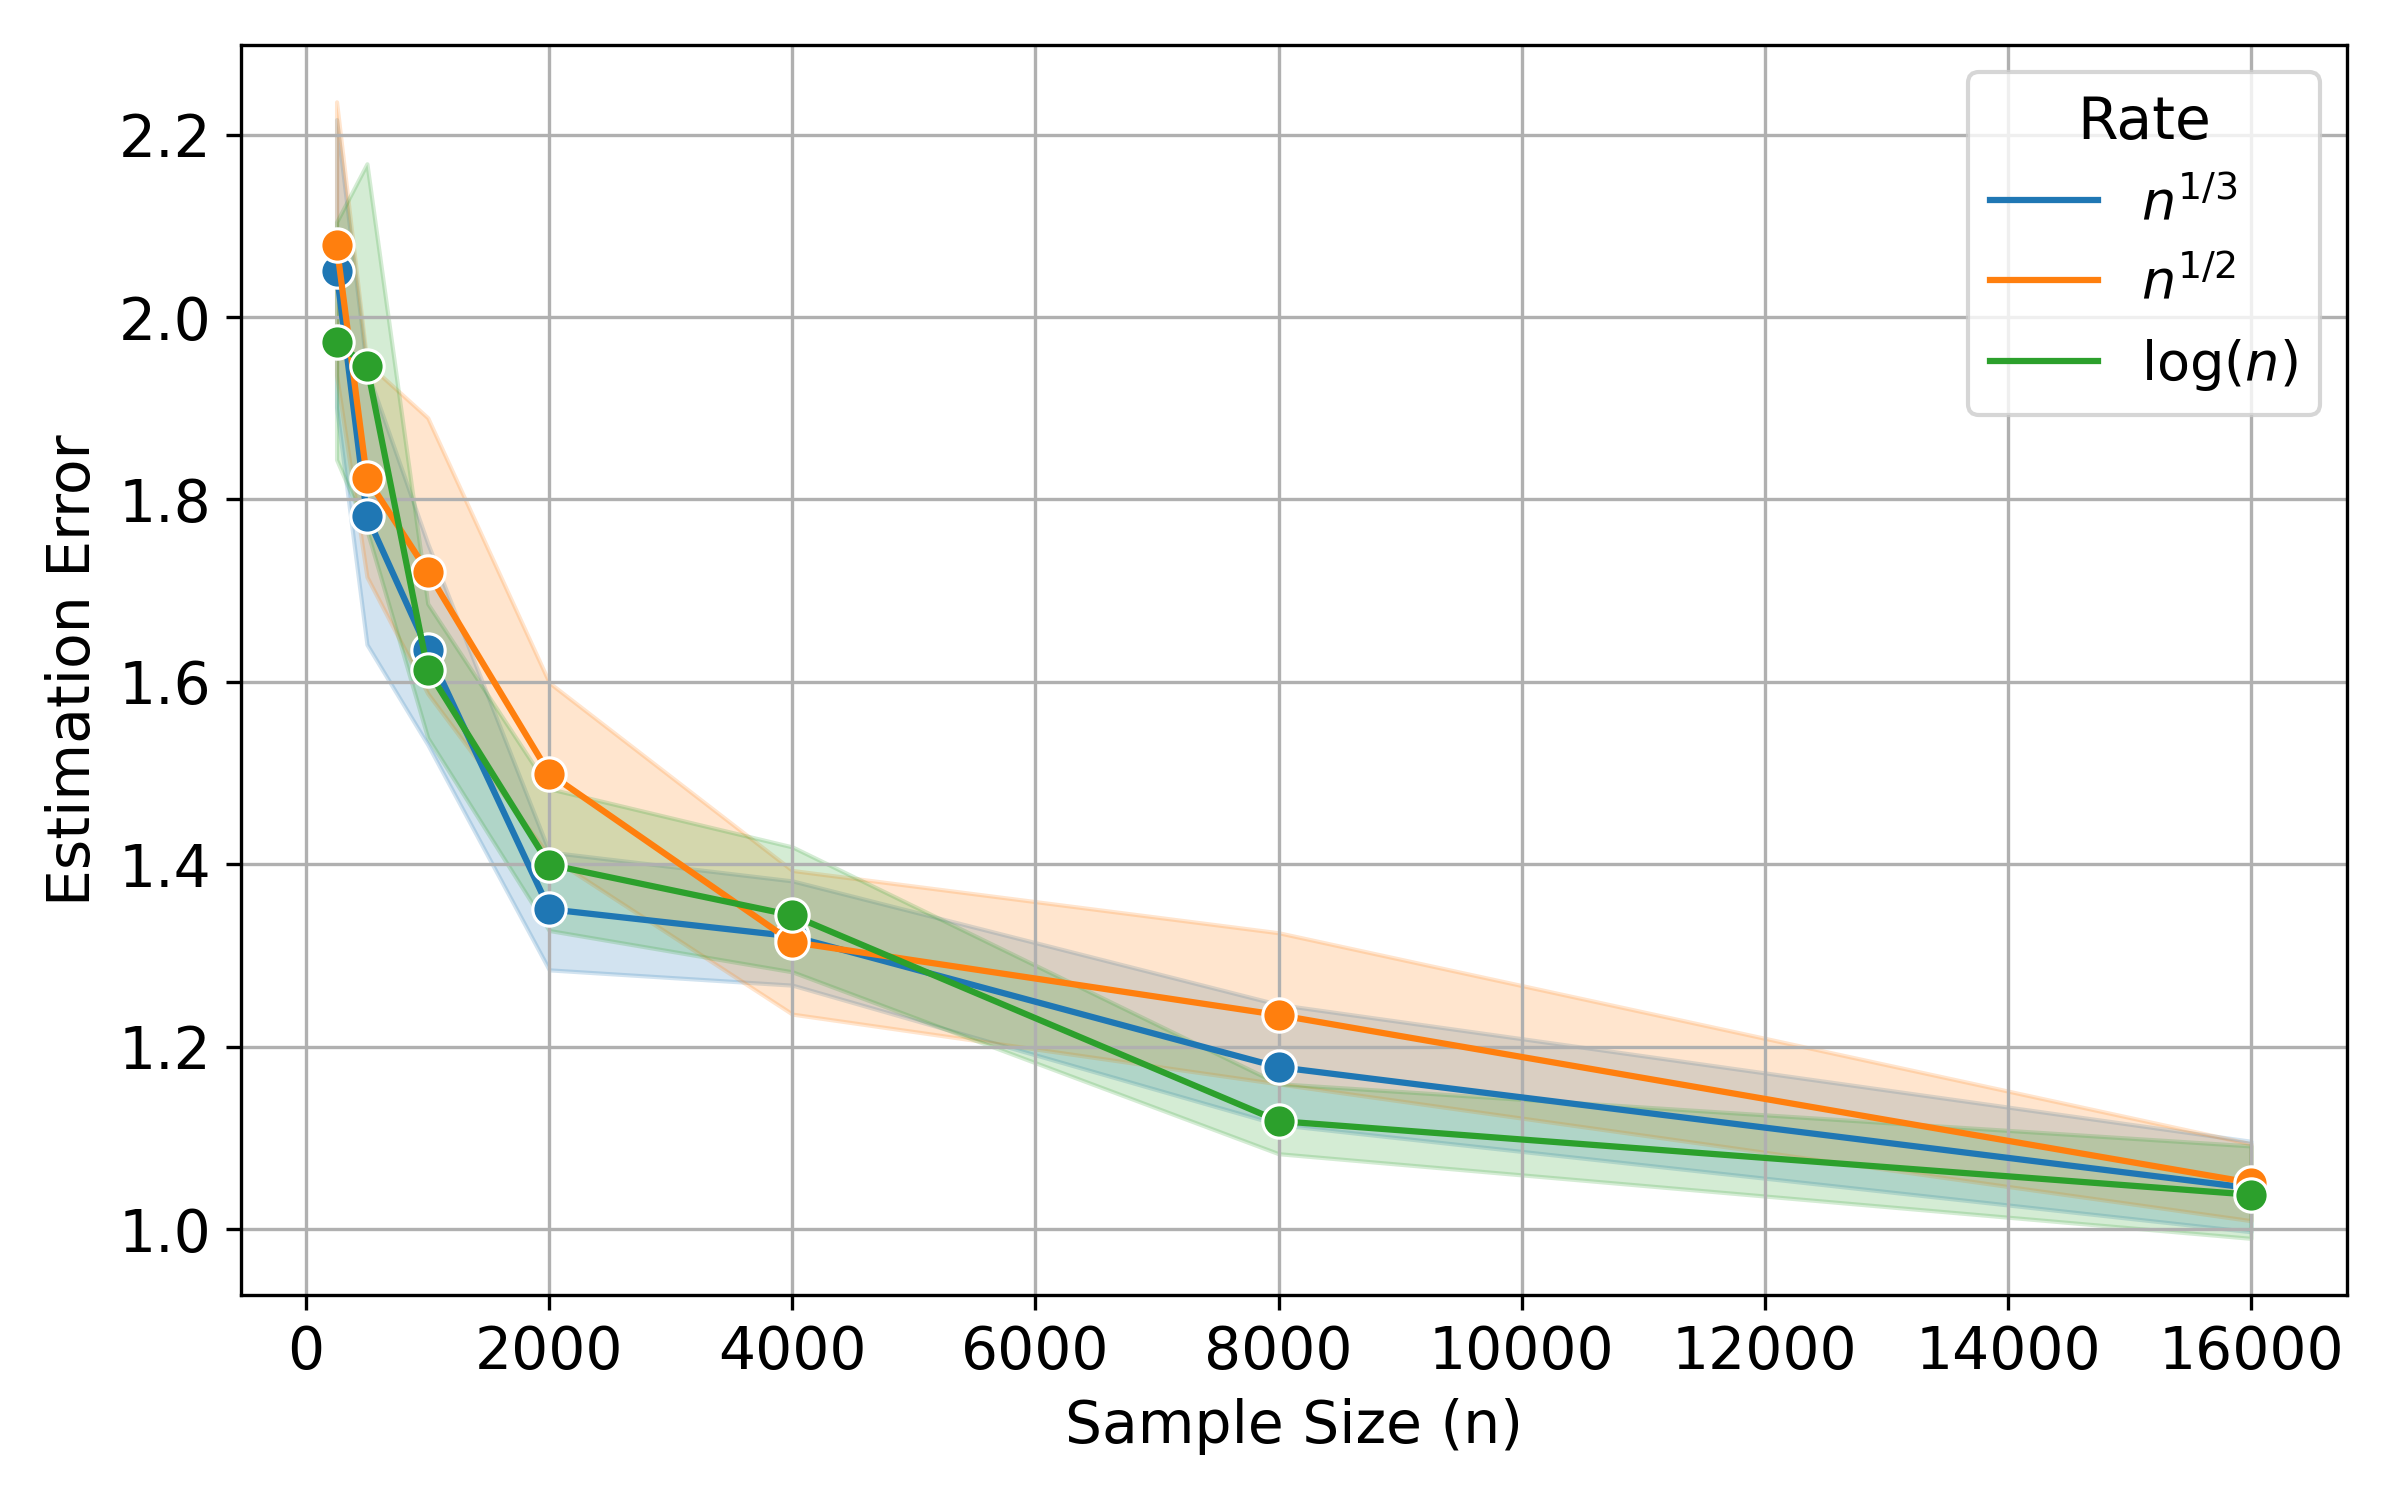
\includegraphics[width=0.65\textwidth]{figs/exp6matrix.png}
\end{figure}
\begin{itemize}
    \item We study the effect of the ratio
    $\rho := \deltastar_{\max} / \deltastar_{\min}$ on the estimation error of $\mMstar$
    using the estimator $\widehat{\mM}_{\mathrm{de}}$.
    \item Experimental setup:
    \begin{itemize}
        \item Fix $\mu = \sqrt{n}\log n$ and $\deltastar_{\min} = \log n$.
        \item Vary $\deltastar_{\max} \in \{\log n,\, n^{1/3},\, n^{1/2}\}$.
    \end{itemize}
    \item Error curves for different values of $\rho$ nearly overlap,
    indicating that $\rho$ has \textbf{negligible impact} on estimation accuracy.
    %\pause
    %\item This suggests that the apparent dependence on
    %$\deltastar_{\max}/\deltastar_{\min}$ in the theory is likely a
    %\textbf{technical artifact}, rather than a fundamental limitation.
\end{itemize}
\end{frame}

\begin{frame}{Linear Forms of Eigenvectors}
\begin{itemize}
    \item Define the eigengap of the $l$-th eigenvalue of $\mMstar$ as 
    \begin{equation*}
        \delta_l^\star := \begin{cases}\min _{1 \leq k \leq r, k \neq l}\left|\lambda_l^{\star}-\lambda_k^{\star}\right|, & \text { if } l>1 \\ \infty & \text { otherwise } .\end{cases}
    \end{equation*}
    \item To estimate the linear form $\va^\top \vustar_l$, \cite{cheng2021tackling} proposes the bias-corrected estimator
    \begin{equation*}
        \widehat{u}_{\boldsymbol{a}, l}:=\min \left\{\sqrt{\left|\frac{\left(\boldsymbol{a}^{\top} \boldsymbol{u}_l\right)\left(\boldsymbol{a}^{\top} \boldsymbol{w}_l\right)}{\boldsymbol{w}_l^{\top} \boldsymbol{u}_l}\right|},\|\boldsymbol{a}\|_2\right\},
    \end{equation*}
    \item \cite{yan2025estimating} shows that under the noise assumption and some assumption on $\lambdastar_{\min}$ and $\delta^\star_{\min}$, with high probability
    \begin{equation*}
        \min \left|\widehat{u}_{\boldsymbol{a}, l} \pm \boldsymbol{a}^{\top} \boldsymbol{u}_l^{\star}\right| \lesssim\left\{\frac{1}{\lambda_{\min }^{\star}}+\max _{k: k \neq l} \frac{\left|\boldsymbol{a}^{\top} \boldsymbol{u}_k^{\star}\right|}{\left|\lambda_l^{\star}-\lambda_k^{\star}\right|}\right\} \sqrt{\sigma^2 \log ^7 n}+\left|\boldsymbol{a}^{\top} \boldsymbol{u}_l^{\star}\right| \frac{\sigma^2 \log ^7 n}{\left(\delta_l^{\star}\right)^2}
    \end{equation*}
    which matches the minimax rate up to log-factors \citep{cheng2021tackling}. 
    \item Taking $\va$ to be the standard basis and using a union bound, \cite{yan2025estimating} shows that 
    $$
    \min \left\|\widehat{\boldsymbol{u}}_l \pm \boldsymbol{u}_l^{\star}\right\|_{\infty} = \tilde{O}\left(\frac{\sigma}{\lambdastar_{\min}} + \frac{\sigma}{\delta_l^{\star}} \sqrt{\frac{\mu}{n}}\right)
    $$
\end{itemize}
\end{frame}


\begin{frame}{Subspace Estimation under $\ell_{2,\infty}$}
\begin{itemize}
    \item Suppose that $\kappa, r = O(1)$, \cite{chen2021spectral} shows that the spectral estimator satisfies
    $$
    \left\|\boldsymbol{U}_\mathrm{sp} \operatorname{sgn}(\mU^\top_\mathrm{sp} \mUstar)-\boldsymbol{U}^{\star}\right\|_{2, \infty} = \tilde{O}\left(\frac{\sigma \sqrt{\mu}}{\lambdastar_{\min}}\right),
    $$
    \item By combining the bias-corrected eigenvectors into a subspace estimator $\widehat{\mU}$, \cite{yan2025estimating} shows that 
    $$
    \min _{\substack{\boldsymbol{S}=\operatorname{diag}\left(s_1, s_2, \ldots, s_r\right), s_l \in\{-1,1\}, l \in[r]}}\left\|\widehat{\boldsymbol{U}} \boldsymbol{S}-\boldsymbol{U}^{\star}\right\|_{2, \infty} = \tilde{O}\left(\sigma\left\{\frac{1}{\lambda_{\min }^{\star}}+\frac{\sqrt{\mu / n}}{\delta_{\min }^{\star}}\right\} \right).
    $$
\end{itemize}
\end{frame}


\end{document}